\documentclass[11pt,a4paper,leqno]{extarticle}
\usepackage[margin=1in]{geometry}
\usepackage[utf8]{inputenc}
\usepackage{booktabs} % for toprule, midrule and bottomrule
\usepackage{adjustbox}
\usepackage{amsmath}
\usepackage{bbold}
\usepackage{etoolbox}
\usepackage{setspace} % for \onehalfspacing and \singlespacing macros
\usepackage[hidelinks]{hyperref}
\usepackage{array}
\usepackage{graphicx}
\usepackage{setspace}
\usepackage{caption}
\usepackage{pdflscape}
\usepackage{caption}
\usepackage{tabularx}
\usepackage{authblk}
\usepackage{float}
\usepackage{siunitx}
\usepackage{titlesec}
\usepackage{pgfplots}
\usepackage[authoryear]{natbib}
\usepackage{scrextend}
\usepackage{nicefrac}
\usepackage{enumitem}
\usepackage{multirow}
\usepackage{xcolor}
\usepackage{cleveref}
\usepackage{varwidth}
\usepackage{gensymb}
\usepackage{lineno}

% section headings
\renewcommand{\thesection}{\Roman{section}.\hspace{-0.5em}}
\renewcommand\thesubsection{\Alph{subsection}.\hspace{-0.5em}}
\renewcommand\thesubsubsection{\hspace{-1em}}
\newcommand{\subsubsubsection}[1]{\begin{center}{\textit{#1}}\end{center}}

\titleformat{\section}
{\bf\centering\large}{\thesection}{1em}{}
\titleformat{\subsection}
{\itshape\centering}{\thesubsection}{1em}{}
\titleformat{\subsubsection}
{\bf}{\thesubsubsection}{1em}{}

% section referencing
\crefformat{section}{\S#2#1#3}
\crefformat{subsection}{\S#2#1#3}
\crefformat{subsubsection}{\S#2#1#3}
\crefrangeformat{section}{\S\S#3#1#4 to~#5#2#6}
\crefmultiformat{section}{\S\S#2#1#3}{ and~#2#1#3}{, #2#1#3}{ and~#2#1#3}

% appendix caption numbering
\DeclareCaptionLabelFormat{AppendixATable}{Table A.#2}
\DeclareCaptionLabelFormat{AppendixBFigure}{Figure B.#2}


% multiline cells
\newcommand{\specialcell}[2][c]{%
	\begin{tabular}[#1]{@{}c@{}}#2\end{tabular}}

% proper caption centering
\DeclareCaptionFormat{centerproper}{%
	% #1: label (e.g. "Table 1")
	% #2: separator (e.g. ": ")
	% #3: caption text
	\begin{varwidth}{\linewidth}%
		\centering
		#1#2#3%
	\end{varwidth}%
}

% caption set up
\captionsetup[table]{
	font = {sc},
	labelfont = {bf}
}

% caption set up
\captionsetup[figure]{
	font = {sc},
	labelfont = {bf}
}

% math claims
\newtheorem{theorem}{Theorem}
\newtheorem{corollary}[theorem]{Corollary}
\newtheorem{proposition}{Proposition}
\newtheorem{lemma}{Lemma}

\newenvironment{proof}[1][Proof]{\noindent\textbf{#1:} }{\ \rule{0.5em}{0.5em}}

%math shortcuts
\DeclareMathOperator*{\argmax}{arg\,max}
\DeclareMathOperator*{\argmin}{arg\,min}

% hyperlinks
\definecolor{darkblue}{RGB}{0,0,150}
\hypersetup{
	colorlinks=true,
	linkcolor = darkblue,
	urlcolor  = darkblue,
	citecolor = darkblue,
	anchorcolor = darkblue
}

% bibliography
\makeatletter
\renewenvironment{thebibliography}[1]
{\section{References}%
	\@mkboth{\MakeUppercase\refname}{\MakeUppercase\refname}%
	\list{}%
	{\setlength{\labelwidth}{0pt}%
		\setlength{\labelsep}{0pt}%
		\setlength{\leftmargin}{\parindent}%
		\setlength{\itemindent}{-\parindent}%
		\@openbib@code
		\usecounter{enumiv}}%
	\sloppy
	\clubpenalty4000
	\@clubpenalty \clubpenalty
	\widowpenalty4000%
	\sfcode`\.\@m}
{\def\@noitemerr
	{\@latex@warning{Empty `thebibliography' environment}}%
	\endlist}
\makeatother

% etoolbox
\AtBeginEnvironment{quote}{\singlespacing}


%% line numbers
%\linenumbers

\begin{document}
	
	\title{\singlespacing{\textbf{Non-Constant Elasticity of Substitution and Intermittent Renewable Energy}}\\\vspace{1em}
	Appendix}
	
	\author[]{Saketh Aleti\thanks{Saketh Aleti: Graduate Student, Department of Economics, Duke University, 419 Chapel Drive, 213 Social Sciences Bldg., Durham, NC 27708-0097, USA (email: saketh.aleti@duke.edu).}  \, and  Gal Hochman\thanks{ Gal Hochman: Professor, Department of Agriculture, Food \& Resource Economics, Rutgers University, 116 Cook Office Building, 55 Dudley Road, New Brunswick, NJ 08901, USA (email: gal.hochman@rutgers.edu).}}
	
%	\date{\vspace{-1em}}
	
	\maketitle
	
%	% Syntax: \begin{addmargin}[<left indentation>]{<indentation>}
%	\begin{addmargin}[0.5in]{0.5in}
%		\textit{In this paper, we present a model of the electricity sector where generation technologies are intermittent. The economic value of an electricity generation technology is given by integrating its production profile with the market price of electricity. We use estimates of the consumer's intertemporal elasticity of substitution for electricity consumption while  parameterizing the model empirically to numerically calculate the elasticity between renewables and fossil energy. We find that there is a non-constant elasticity of substitution between renewable and fossil energy that depends on prices and intermittency. This suggests that the efficacy and welfare effects of carbon taxes and renewable subsidies vary geographically. Subsidizing research into battery technology and tailoring policy for local energy markets can mitigate these distributional side effects while complementing traditional policies used to promote renewable energy. 
%		}
%		\\
%		\noindent\textbf{Key words:} renewable energy, intermittency, pollution, environment
%		
%		\noindent\textbf{JEL Classifications:} Q28, Q41, Q48, Q52, Q55, Q58
%	\end{addmargin}
%	
	
	
	
	
	

	
	\section{Appendix A: Supplementary Proofs}
	\label{sec:appendixa}
	
	\renewcommand{\theequation}{\arabic{equation}a}
	
	
	\subsection{Cobb-Douglas Case with Two Periods \& Two Technologies}
	\label{sec:cobbdoug}
	
	In this section, we consider a simpler case of our general model to better understand its implications. Firstly, we restrict the utility function to its Cobb-Douglas form which is simply the case where the elasticity of substitution $\sigma = 1$. Secondly, we limit the number of periods and technologies to 2. And, thirdly, we normalize the prices such that our representative consumer's income $I$ is $1$.
	
	\subsubsection{Equilibrium Results}
	
	Firstly, our demand equations simplify to:
	\begin{align}
	Z_t &= \alpha_t / p_t \\
	Z_s &= \alpha_s / p_s
	\end{align}
	where $t$ and $s$ are our two periods. Next, solving for the FOC condition for profit maximization, we have:
	\begin{align}
	\mathbf{p} &=  \boldsymbol{\xi}^{-1} \mathbf{c} = \begin{pmatrix}
	-\dfrac{c_{1}\,\xi _{\mathrm{2s}}-c_{2}\,\xi _{\mathrm{1s}}}{\xi _{\mathrm{1s}}\,\xi _{\mathrm{2t}}-\xi _{\mathrm{1t}}\,\xi _{\mathrm{2s}}}  \\[2ex]
	\dfrac{c_{1}\,\xi _{\mathrm{2t}}-c_{2}\,\xi _{\mathrm{1t}}}{\xi _{\mathrm{1s}}\,\xi _{\mathrm{2t}}-\xi _{\mathrm{1t}}\,\xi _{\mathrm{2s}}} 
	\end{pmatrix} 
	\end{align}
	And, substituting back into our demand equations, we find the equilibrium quantities for $\mathbf{Z}$ and $\mathbf{X}$. 
	\begin{align}
	\mathbf{Z} &= \begin{pmatrix}
	\dfrac{\alpha _{t}\,\left(\xi _{\mathrm{1s}}\,\xi _{\mathrm{2t}}-\xi _{\mathrm{1t}}\,\xi _{\mathrm{2s}}\right)}{c_{2}\,\xi _{\mathrm{1s}} - c_{1}\,\xi _{\mathrm{2s}}} \\[2ex]
	\dfrac{\alpha _{s}\,\left(\xi _{\mathrm{1s}}\,\xi _{\mathrm{2t}}-\xi _{\mathrm{1t}}\,\xi _{\mathrm{2s}}\right)}{c_{1}\,\xi _{\mathrm{2t}}-c_{2}\,\xi _{\mathrm{1t}}} 
	\end{pmatrix}\\
	\implies 
	\mathbf{X} &= \begin{pmatrix}
	\dfrac{\alpha _{t}\,\xi _{\mathrm{2s}}}{c_{1}\,\xi _{\mathrm{2s}}-c_{2}\,\xi _{\mathrm{1s}}}+\dfrac{\alpha _{s}\,\xi _{\mathrm{2t}}}{c_{1}\,\xi _{\mathrm{2t}}-c_{2}\,\xi _{\mathrm{1t}}} \\[2ex] 
	-\dfrac{\alpha _{t}\,\xi _{\mathrm{1s}}}{c_{1}\,\xi _{\mathrm{2s}}-c_{2}\,\xi _{\mathrm{1s}}}-\dfrac{\alpha _{s}\,\xi _{\mathrm{1t}}}{c_{1}\,\xi _{\mathrm{2t}}-c_{2}\,\xi _{\mathrm{1t}}}
	\end{pmatrix}
	\end{align}
	We now derive the restrictions on the parameters $\boldsymbol{\xi}$ and $\mathbf{c}$ that ensure $\mathbf{Z}, \mathbf{X} > 0$. These restrictions are given by Lemma 1 from the Model Equilibrium section:
	
	\hfill
	
	\noindent	\textbf{Lemma 1A:} \textit{ Assume that, for all technologies $i$ and periods $t$, we have $\xi_{i,t} > 0 \, , \alpha_t > 0 \, ,$ and $ c_i > 0$. Then, for technology $j$ to be economical, there need to exist a period $s$ where the following three conditions are met:
		\begin{itemize}
			\item $\xi_{j,s}/c_j > \xi_{i,s}/c_i$ for all $i$
			\item $\xi_{j,s}/\xi_{j,t} >  \xi_{i,s}/\xi_{i,t} $ where $i \neq j$ and $t \neq s$
			\item Period $s$ demand needs to be sufficiently large, i.e., $\alpha_s$ is large enough
		\end{itemize}
	}
	
	In order to have $X_1, X_2 > 0$, we need to have the conditions of this lemma hold for both technologies. This is equivalent to  requiring one of two possible sets of symmetrical restrictions on $\boldsymbol{\xi}$ and $\mathbf{c}$ which are detailed in \autoref{tab:paramrest}. The first set, Case 1, assumes that technology 2 is more cost efficient in period $t$, while the second set, Case 2, assumes that technology 1 is more cost efficient in period $t$. If a given set of parameters do not fall into either case, we are left with an edge case where one of the technologies is not used. Additionally, these inequalities compare two types of efficiency -- output efficiency and cost efficiency; we define output efficiency as electricity output per unit of input and cost efficiency in terms of electricity output per dollar of input. We refer to the last set of restrictions as mixed, because they relate both cost and output efficiency. 


	\vspace{0.15in}
	\begin{center}
		[INSERT Table A.1: Parameter Restrictions for $\mathbf{Z}, \mathbf{X} > 0$]
	\end{center}
	\vspace{0.15in}
	

	\begin{proof}
		We aim to derive conditions on $\xi$ and $c$ required to have positive $\mathbf{Z}$ and $\mathbf{X}$, so we begin by assuming $\mathbf{Z}, \mathbf{X} > 0$. Second, since the equations so far are symmetrical, note that there be two symmetrical sets of potential restrictions we must impose on the parameters. Thus, we first assume the inequality $c_1 \xi_{2t} - c_2 \xi_{1t} > 0$ to restrict ourselves to one of the two cases. This assumption results in the denominator of $Z_s$ being positive. Hence, we must also have $\xi_{1s}\xi_{2t} - \xi_{2s}\xi_{1t} > 0 $ for $Z_s > 0$. This same term appears in the numerator for $Z_t$, hence its denominator must be positive: $c_2 \xi_{1s} - c_1 \xi_{2s} > 0$. Now, rewriting these inequalities, we have:
		\begin{align*}
		c_1 \xi_{2t} - c_2 \xi_{1t} > 0 &\implies \xi_{2t}/c_2 > \xi_{1t}/c_1 \\
		c_2 \xi_{1s} - c_1 \xi_{2s} > 0 &\implies \xi_{1s}/c_1 > \xi_{2s}/c_2 \\
		\xi_{1s}\xi_{2t} - \xi_{2s}\xi_{1t} > 0 &\implies \xi_{1s}/\xi_{1t} > \xi_{2s}/\xi_{2t} \\
		&\implies \xi_{1t}/\xi_{1s} < \xi_{2t}/\xi_{2s} 
		\end{align*}
		Note that the latter two restrictions can be derived from the former two. Additionally, we implicitly assume that we have $\boldsymbol{\xi} > 0$. However, this is not necessary assumption, since $\boldsymbol{\xi}$ invertible only requires $\xi_{1t} \xi_{2s} > 0$ or $\xi_{1s} \xi_{2t} > 0$. Instead, we may leave the latter two inequalities in the form $ \xi_{1s}\xi_{2t} > \xi_{2s}\xi_{1t}$ which remains valid when values of $\xi$ are equal to $0$. Lastly, the mixed efficiency restrictions come from $X > 0$. To start, for $X_1$, we have:
		\begin{align*}
		X_1 > 0 &\implies (\alpha_t \xi_{2s})(c_1 \xi_2t - c_2\xi_1t) + (\alpha_s \xi_{2t})(c_1 \xi_{2s} - c_2 \xi_{1s}) < 0\\
		&\implies (\alpha_t \xi_{2s})(c_1 \xi_2t - c_2\xi_1t) < (\alpha_s \xi_{2t})(c_2 \xi_{1s} - c_1 \xi_{2s}) \\
		&\implies (\xi_{2s}/\xi_{2t}) < (\alpha_s (c_2 \xi_{1s} - c_1 \xi_{2s}))/(\alpha_t(c_1 \xi_{2t} - c_2\xi_{1t})) \\
		&\implies (\xi_{2s}/\xi_{2t}) < (\alpha_s (\xi_{1s}/c_1 -  \xi_{2s}/c_2))/(\alpha_t(\xi_{2t}/c_2 - \xi_{1t}/c_1)) 
		\end{align*}
		Similarly, for $X_2$, note that only the numerators differ; $\xi_{2s}$ is replaced with $-\xi_{1s}$ and $\xi_{2t}$ is replaced with $-\xi_{1t}$. Hence, we have
		\begin{align*}
		X_2 > 0 &\implies (\alpha_t \xi_{1s})(c_1 \xi_2t - c_2\xi_1t) + (\alpha_s \xi_{1t})(c_1 \xi_{2s} - c_2 \xi_{1s}) > 0\\
		&\implies (\xi_{1s}/\xi_{1t}) > (\alpha_s (\xi_{1s}/c_1 -  \xi_{2s}/c_2))/(\alpha_t(\xi_{2t}/c_2 - \xi_{1t}/c_1)) 
		\end{align*}
		To double check, note that combining the inequalities from $X_1>0$ and $X_2 > 0$ leads to $\xi_{2s}/\xi_{2t} < \xi_{1s}/\xi_{1t}$. This is precisely the earlier result obtained from $\mathbf{Z} > 0$. Again, it is  important to note that we assume $\boldsymbol{\xi} > 0$ for to simplify the inequalities of $X_1 > 0$ and $X_2 > 0$ . Otherwise, we may leave the inequalities in their original forms and they are still valid when  $\xi_{1t} \xi_{2s} > 0$ or $\xi_{1s} \xi_{2t} > 0$.   \\ \hfill
	\end{proof}
	
	Let us consider the set of restrictions belonging to Case 1. The first inequality, our initial assumption, states that technology 2 is relatively more cost efficient in period $t$. The second inequality claims technology 1 is relatively more cost efficient in period $s$. The implications are fairly straightforward; if a technology is to be used, it must have an absolute advantage in cost efficiency in at least one period. The third condition states that the relative output efficiency of technology 2 is greater than that of the first technology in period $t$. And, the fourth condition makes a symmetrical claim but for the technology 1 and period $s$. These latter two restrictions regarding output efficiency enter $\mathbf{Z}$ and $\mathbf{X}$ through $\mathbf{p}$; they're simply a restatement of the invertibility of $\xi$ and can also be derived through the cost efficiency restrictions. 
	
	The mixed efficiency restrictions are less intuitive. Firstly, note that $\left(\xi_{1s}/c_1 - \xi_{2s}/c_2\right)$ is the difference in cost efficiency for the two technologies in period $s$; this is equivalent to the increase in $Z_s$ caused by shifting a marginal dollar towards technology 1. Similarly, the bottom term $\left( \xi_{2t}/c_2 - \xi_{1t}/c_1 \right)$ represents the change in $Z_t$ caused by shifting a marginal dollar towards technology 1. Both these terms are then multiplied by the share parameter of the utility function for their respective time periods. Furthermore, note that $\alpha_t$ $(\alpha_s)$ is the elasticity of utility with respect to $Z_t$ $(Z_s)$. Hence, in total, the mixed efficiency restrictions relate the relative cost efficiencies of each technology with their output efficiency and the demand for energy. So, for example, suppose that consumers prefer, \textit{ceteris paribus}, that nearly all their electricity arrives in period $t$. This would imply $\alpha_t$ is arbitrarily large which results in the left-hand side of the fraction becoming arbitrarily small. This violates the first mixed efficiency restriction but not the second; consequently, use of the first technology, which is less cost efficient in period $t$, approaches $0$. 
	
	
	
	In more practical terms, suppose that our first technology is coal power and the latter is solar power. Although coal power is dispatchable, it does not easily ramp up or down within a day; hence, it is reasonable to apply our model where capacities are fixed over time so long as our time frame is sufficiently short. Hence, we now assume periods $t$ and $s$ represent the peak and off-peak for a day. And, we expect that there is more available solar radiation during peak hours than off-peak hours, since peak hours are usually during the middle of the day. This implies that the output efficiency of solar power is higher in period $t$ due to more available solar radiation. Additionally, since the energy output of a unit of coal is independent of time, we know that the output efficiency of coal is constant. In total, this implies that we have met the output efficiency restrictions, since we have $\xi_{2t}/\xi_{2s} > \xi_{1t}/\xi_{1s}$. Next, we can reasonably assume that coal is more cost efficient than solar in the off-peak period when there is less sun; hence, the second cost efficiency restriction is satisfied. Then, for there to be an incentive to use solar power, we must satisfy the first cost-efficiency condition; that is, solar needs be cost efficient during peak hours otherwise we hit an edge case where no solar is employed. And, finally, solar must also satisfy the mixed efficiency condition, which essentially implies that there must be sufficient demand for electricity during period $t$, when solar is more effective, for it to be a feasible technology. So, overall, for a technology to be economical, it must meet three conditions: it must the most cost efficient technology for a particular period, it must have a comparative advantage in output efficiency in the same period, and there must be a sufficient amount of demand in that period. 
	
	
	%\footnote{This same analysis can be further extended to any $n$ technologies. However, the number restrictions and different cases to ensure $X , Z > 0$ expands very quickly ($O(n!)$). For instance, if we had 3 technologies and 3 periods, we must first assume each technology is more cost efficient than the other two in a unique period; this adds 3*2 restrictions. Then, we must make the output efficiency restrictions comparing each pair of technologies for each pair of periods.} 
	
	\subsubsection{Comparative Statics}
	
	
	The comparative statics are similarly intuitive. The equilibrium quantity of a technology is increasing with its output efficiency and decreasing with its cost per unit. Additionally, the equilibrium quantities for a particular technology move in the opposite direction with respect to the output efficiency and cost of the other technologies. For a practical example, consider again coal and solar power from before. An increase in the output efficiency of solar or a decrease in solar power's cost will reduce the optimal quantity of coal power. Likewise, as coal power's efficiency improves, it's adoption rises. To find the effects of $\boldsymbol{\alpha}$ on $\mathbf{X}$, we must assume one of the cases of restrictions shown in  \autoref{tab:paramrest}. So, again, let us assume Case 1 is true; this implies that $X_2$ is the most cost efficient technology in period $t$ and likewise for $X_1$ in period $s$. Firstly, note that $\boldsymbol{\alpha}$ determines the demand for electricity in a period. Hence, when $\alpha_t$ rises, we see the optimal level of $X_2$ rise as well; likewise, $X_1$ rises with $\alpha_s$. In short, the optimal quantity of a technology rises linearly with the demand for electricity in the period it specializes in. Moreover, these relationships are reversed with respect to demand in each technology's suboptimal period. So, for example, we would expect the use of solar energy to rise when the demand for electricity during peak hours rises, and it would fall when demand for energy in the off-peak rises. On the other hand, use coal power would rise with off-peak demand and fall with peak demand. This concept carries through for the comparative statics of $\mathbf{Z}$. When the output efficiency of technology 1 rises or its cost falls, we see output $Z_s$ rise and output $Z_t$ fall. This is because technology 1 is optimal in period $s$ given the Case 1 restrictions. Likewise, we see symmetrical results for the output with respect to the cost and output efficiency of technology 2; improvements in the efficiency of $X_2$ result in greater output in $Z_t$ and smaller output in $Z_s$.  In total, we have Proposition 1:
	
	\hfill
	
	\noindent	\textbf{Proposition 1A:} \textit{Suppose that the conditions of Lemma 1 hold for each technology, so we are not in an edge case. Then, 
		\begin{itemize}
			\item The equilibrium quantity of a technology is increasing with its output and decreasing with its cost; at the same time, it is decreasing with the output of other technologies and increasing with the cost of other technologies. 
			\item Also, suppose that some technology $i$ is the most cost efficient in period $t$. Then, its equilibrium quantity is increasing with respect to the demand parameter $\alpha_t$ and decreasing with respect to the demand parameters in other periods. 
			\item Furthermore, again assuming technology $i$ is the most cost efficient in period $t$, the comparative statics of $Z_t$ and $X_i$ are equivalent. 
	\end{itemize}}
	
	
	\hfill 
	
	\begin{proof}
		We begin by deriving the comparative statics of the cost and efficiency parameters with respect to $\mathbf{X}$.   Firstly, we take derivatives with respect to the cost vectors:
		\begin{align*}
		\frac{\partial X_1}{\partial \mathbf{c}} &= 
		\begin{pmatrix}
		\dfrac{-\alpha _{t}\,{\xi _{\mathrm{2s}}}^2}{{\left(c_{1}\,\xi _{\mathrm{2s}}-c_{2}\,\xi _{\mathrm{1s}}\right)}^2}-\dfrac{\alpha _{s}\,{\xi _{\mathrm{2t}}}^2}{{\left(c_{1}\,\xi _{\mathrm{2t}}-c_{2}\,\xi _{\mathrm{1t}}\right)}^2}<0 \\
		\dfrac{\alpha _{t}\,\xi _{\mathrm{1s}}\,\xi _{\mathrm{2s}}}{{\left(c_{1}\,\xi _{\mathrm{2s}}-c_{2}\,\xi _{\mathrm{1s}}\right)}^2}+\dfrac{\alpha _{s}\,\xi _{\mathrm{1t}}\,\xi _{\mathrm{2t}}}{{\left(c_{1}\,\xi _{\mathrm{2t}}-c_{2}\,\xi _{\mathrm{1t}}\right)}^2}>0
		\end{pmatrix}\\
		\frac{\partial X_2}{\partial \mathbf{c}} &= 
		\begin{pmatrix}
		\dfrac{\alpha _{t}\,\xi _{\mathrm{1s}}\,\xi _{\mathrm{2s}}}{{\left(c_{1}\,\xi _{\mathrm{2s}}-c_{2}\,\xi _{\mathrm{1s}}\right)}^2}+\dfrac{\alpha _{s}\,\xi _{\mathrm{1t}}\,\xi _{\mathrm{2t}}}{{\left(c_{1}\,\xi _{\mathrm{2t}}-c_{2}\,\xi _{\mathrm{1t}}\right)}^2}>0 \\
		\dfrac{-\alpha _{t}\,{\xi _{\mathrm{1s}}}^2}{{\left(c_{1}\,\xi _{\mathrm{2s}}-c_{2}\,\xi _{\mathrm{1s}}\right)}^2}-\dfrac{\alpha _{s}\,{\xi _{\mathrm{1t}}}^2}{{\left(c_{1}\,\xi _{\mathrm{2t}}-c_{2}\,\xi _{\mathrm{1t}}\right)}^2}<0
		\end{pmatrix}
		\end{align*}
		The first and second terms of $\partial X_1 / \partial c_1$ are clearly both negative independent of the restrictions on the parameters. Similarly, all terms of  $\partial X_1 / \partial c_2$ are positive independent of any restrictions. Since the structure of this problem is symmetrical with respect to $X_1$ and $X_2$, the same comparative statics apply but in reverse for $X_1$. Next, we derive comparative statics for each element of $\xi$.
		\begin{alignat*}{1}
		\frac{\partial X_1}{\partial \boldsymbol{\xi}} &= 
		\begin{pmatrix}
		\dfrac{\alpha _{s}\,c_{2}\,\xi _{\mathrm{2t}}}{{\left(c_{1}\,\xi _{\mathrm{2t}}-c_{2}\,\xi _{\mathrm{1t}}\right)}^2}>0 & \dfrac{\alpha _{t}\,c_{2}\,\xi _{\mathrm{2s}}}{{\left(c_{1}\,\xi _{\mathrm{2s}}-c_{2}\,\xi _{\mathrm{1s}}\right)}^2}>0 \\
		\dfrac{-\alpha _{s}\,c_{2}\,\xi _{\mathrm{1t}}}{{\left(c_{1}\,\xi _{\mathrm{2t}}-c_{2}\,\xi _{\mathrm{1t}}\right)}^2}<0 & \dfrac{-\alpha _{t}\,c_{2}\,\xi _{\mathrm{1s}}}{{\left(c_{1}\,\xi _{\mathrm{2s}}-c_{2}\,\xi _{\mathrm{1s}}\right)}^2}<0 \\
		\end{pmatrix}\\
		\frac{\partial X_2}{\partial \boldsymbol{\xi}} &= 
		\begin{pmatrix}
		\dfrac{-\alpha _{s}\,c_{1}\,\xi _{\mathrm{2t}}}{{\left(c_{1}\,\xi _{\mathrm{2t}}-c_{2}\,\xi _{\mathrm{1t}}\right)}^2} <0& \dfrac{-\alpha _{t}\,c_{1}\,\xi _{\mathrm{2s}}}{{\left(c_{1}\,\xi _{\mathrm{2s}}-c_{2}\,\xi _{\mathrm{1s}}\right)}^2} <0\\
		\dfrac{\alpha _{s}\,c_{1}\,\xi _{\mathrm{1t}}}{{\left(c_{1}\,\xi _{\mathrm{2t}}-c_{2}\,\xi _{\mathrm{1t}}\right)}^2}>0& \dfrac{\alpha _{t}\,c_{1}\,\xi _{\mathrm{1s}}}{{\left(c_{1}\,\xi _{\mathrm{2s}}-c_{2}\,\xi _{\mathrm{1s}}\right)}^2} >0\\
		\end{pmatrix}
		\end{alignat*}
		Again, the signs are fairly straightforward. The optimal quantity of $X_1$ increases with its output efficiency in both periods; however, it decreases with the output efficiency of $X_2$ in both periods. Similarly, symmetrical results are shown for $X_2$. Next, we study the effects of $\boldsymbol{\alpha}$ on $\mathbf{X}$; this requires us to place some restrictions on the parameters, so we use those belonging to Case 1 in \autoref{tab:paramrest}. Then, we have 
		\begin{align*}
		\frac{\partial X_1}{\partial \boldsymbol{\alpha}} &= 
		\begin{pmatrix}
		\dfrac{\xi _{\mathrm{2s}}}{c_{1}\,\xi _{\mathrm{2s}}-c_{2}\,\xi _{\mathrm{1s}}}<0 \\
		\dfrac{\xi _{\mathrm{2t}}}{c_{1}\,\xi _{\mathrm{2t}}-c_{2}\,\xi _{\mathrm{1t}}}>0
		\end{pmatrix}\\
		\frac{\partial X_2}{\partial \boldsymbol{\alpha}} &= 
		\begin{pmatrix}
		\dfrac{-\xi _{\mathrm{1s}}}{c_{1}\,\xi _{\mathrm{2s}}-c_{2}\,\xi _{\mathrm{1s}}}>0 \\
		\dfrac{-\xi _{\mathrm{1t}}}{c_{1}\,\xi _{\mathrm{2t}}-c_{2}\,\xi _{\mathrm{1t}}}<0
		\end{pmatrix}
		\end{align*}
		Note that our restrictions imply that $c_1 \xi_{2t} - c_2 \xi_{1t} > 0$ and $c_2 \xi_{1s} - c_1 \xi_{2s} > 0$. From here, the intuition is clear; we assume that $X_2$ is more cost efficient in period $t$, so increases in demand during period $t$ (caused by increases in $\alpha_t$) will increase the optimal quantity of $X_2$. And, the same applies to $X_1$ with respect to period $s$ and $\alpha_s$. Again, due to symmetry, the statics are reversed when the technologies are flipped. Similarly, the signs would also be flipped if we used the restrictions given by Case 2 instead. 
		
		Next, we derive the comparative statics for $\mathbf{Z}$. From our restrictions, we have $\xi_{1s}\xi_{2t} > \xi_{2s}\xi_{1t}$. All the results above follow from this inequality and the cost efficiency restrictions. 
		\begin{align*}
		\frac{\partial Z_t}{\partial \mathbf{c}} &= 
		\begin{pmatrix}
		\dfrac{\alpha _{t}\,\xi _{\mathrm{2s}}\,\left(\xi _{\mathrm{1s}}\,\xi _{\mathrm{2t}}-\xi _{\mathrm{1t}}\,\xi _{\mathrm{2s}}\right)}{{\left(c_{1}\,\xi _{\mathrm{2s}}-c_{2}\,\xi _{\mathrm{1s}}\right)}^2}>0\\
		\dfrac{-\alpha _{t}\,\xi _{\mathrm{1s}}\,\left(\xi _{\mathrm{1s}}\,\xi _{\mathrm{2t}}-\xi _{\mathrm{1t}}\,\xi _{\mathrm{2s}}\right)}{{\left(c_{1}\,\xi _{\mathrm{2s}}-c_{2}\,\xi _{\mathrm{1s}}\right)}^2}<0
		\end{pmatrix}\\
		\frac{\partial Z_s}{\partial \mathbf{c}} &= 
		\begin{pmatrix}
		\dfrac{-\alpha _{s}\,\xi _{\mathrm{2t}}\,\left(\xi _{\mathrm{1s}}\,\xi _{\mathrm{2t}}-\xi _{\mathrm{1t}}\,\xi _{\mathrm{2s}}\right)}{{\left(c_{1}\,\xi _{\mathrm{2t}}-c_{2}\,\xi _{\mathrm{1t}}\right)}^2} <0\\
		\dfrac{\alpha _{s}\,\xi _{\mathrm{1t}}\,\left(\xi _{\mathrm{1s}}\,\xi _{\mathrm{2t}}-\xi _{\mathrm{1t}}\,\xi _{\mathrm{2s}}\right)}{{\left(c_{1}\,\xi _{\mathrm{2t}}-c_{2}\,\xi _{\mathrm{1t}}\right)}^2} >0
		\end{pmatrix}\\
		\frac{\partial Z_t}{\partial \boldsymbol{\xi}} &= 
		\begin{pmatrix}
		\dfrac{\alpha _{t}\,\xi _{\mathrm{2s}}}{c_{1}\,\xi _{\mathrm{2s}}-c_{2}\,\xi _{\mathrm{1s}}} < 0& \dfrac{-\alpha _{t}\,\xi _{\mathrm{2s}}\,\left(c_{1}\,\xi _{\mathrm{2t}}-c_{2}\,\xi _{\mathrm{1t}}\right)}{{\left(c_{1}\,\xi _{\mathrm{2s}}-c_{2}\,\xi _{\mathrm{1s}}\right)}^2} <0 \\
		\dfrac{-\alpha _{t}\,\xi _{\mathrm{1s}}}{c_{1}\,\xi _{\mathrm{2s}}-c_{2}\,\xi _{\mathrm{1s}}} >0& \dfrac{\alpha _{t}\,\xi _{\mathrm{1s}}\,\left(c_{1}\,\xi _{\mathrm{2t}}-c_{2}\,\xi _{\mathrm{1t}}\right)}{{\left(c_{1}\,\xi _{\mathrm{2s}}-c_{2}\,\xi _{\mathrm{1s}}\right)}^2} >0\\
		\end{pmatrix}\\
		\frac{\partial Z_s}{\partial \boldsymbol{\xi}} &= 
		\begin{pmatrix}
		\dfrac{-\alpha _{s}\,\xi _{\mathrm{2t}}\,\left(c_{1}\,\xi _{\mathrm{2s}}-c_{2}\,\xi _{\mathrm{1s}}\right)}{{\left(c_{1}\,\xi _{\mathrm{2t}}-c_{2}\,\xi _{\mathrm{1t}}\right)}^2}> 0& \dfrac{\alpha _{s}\,\xi _{\mathrm{2t}}}{c_{1}\,\xi _{\mathrm{2t}}-c_{2}\,\xi _{\mathrm{1t}}} > 0\\
		\dfrac{\alpha _{s}\,\xi _{\mathrm{1t}}\,\left(c_{1}\,\xi _{\mathrm{2s}}-c_{2}\,\xi _{\mathrm{1s}}\right)}{{\left(c_{1}\,\xi _{\mathrm{2t}}-c_{2}\,\xi _{\mathrm{1t}}\right)}^2} < 0& \dfrac{-\alpha _{s}\,\xi _{\mathrm{1t}}}{c_{1}\,\xi _{\mathrm{2t}}-c_{2}\,\xi _{\mathrm{1t}}} <0\\
		\end{pmatrix}
		\end{align*}
		Again, recall that we have $c_1 \xi_{2t} - c_2 \xi_{1t} > 0$ and $c_2 \xi_{1s} - c_1 \xi_{2s} > 0$; the rest follows. And finally, we have:
		\begin{align*}
		\frac{\partial Z_t}{\partial \boldsymbol{\alpha}} &= 
		\begin{pmatrix}
		\dfrac{-\xi _{\mathrm{1s}}\,\xi _{\mathrm{2t}}-\xi _{\mathrm{1t}}\,\xi _{\mathrm{2s}}}{c_{1}\,\xi _{\mathrm{2s}}-c_{2}\,\xi _{\mathrm{1s}}} > 0  \\
		0
		\end{pmatrix} \\
		\frac{\partial Z_s}{\partial \boldsymbol{\alpha}} &= 
		\begin{pmatrix}
		0 \\
		\dfrac{\xi _{\mathrm{1s}}\,\xi _{\mathrm{2t}}-\xi _{\mathrm{1t}}\,\xi _{\mathrm{2s}}}{c_{1}\,\xi _{\mathrm{2t}}-c_{2}\,\xi _{\mathrm{1t}}} > 0
		\end{pmatrix}
		\end{align*}
		These are fairly trivial, since $Z_t = \alpha_t / p_t$ (and $Z_s = \alpha_s/ p_s$) and prices are positive. \\
		\hfill
	\end{proof}
	
	
	\subsubsection{Elasticity of Substitution}
	\label{sec:EOS_derivation}
	
	We derive the elasticity of substitution between technologies in this two-period, two-technology setting. By definition, the elasticity of substitution is 
	\begin{equation}
	e_{12} \equiv \frac{\partial \log(X_1/X_2)}{\partial \log(c_2/c_1)} = \frac{\partial X_1/X_2 }{ \partial (c_2/c_1)} \cdot \frac{c_2/c_1}{X_1/X_2} = \frac{\partial X_1/X_2}{ \partial  c_2}  \cdot \frac{\partial c_2}{\partial (c_2/c_1)} \cdot \frac{c_2/c_1}{X_1/X_2} 
	\end{equation}
	Note that
	\begin{align}
		X_1/X_2 &= -\frac{\alpha _{s}\,c_{1}\,\xi _{\mathrm{2s}}\,\xi _{\mathrm{2t}}-\alpha _{s}\,c_{2}\,\xi _{\mathrm{1s}}\,\xi _{\mathrm{2t}}+\alpha _{t}\,c_{1}\,\xi _{\mathrm{2s}}\,\xi _{\mathrm{2t}}-\alpha _{t}\,c_{2}\,\xi _{\mathrm{1t}}\,\xi _{\mathrm{2s}}}{\alpha _{s}\,c_{1}\,\xi _{\mathrm{1t}}\,\xi _{\mathrm{2s}}-\alpha _{s}\,c_{2}\,\xi _{\mathrm{1s}}\,\xi _{\mathrm{1t}}+\alpha _{t}\,c_{1}\,\xi _{\mathrm{1s}}\,\xi _{\mathrm{2t}}-\alpha _{t}\,c_{2}\,\xi _{\mathrm{1s}}\,\xi _{\mathrm{1t}}} \\
		\frac{\partial X_1/X_2}{\partial c_2} &= \frac{\alpha _{s}\,\alpha _{t}\,c_{1}\,{\left(\xi _{\mathrm{1s}}\,\xi _{\mathrm{2t}}-\xi _{\mathrm{1t}}\,\xi _{\mathrm{2s}}\right)}^2}{{\left(\alpha _{s}\,c_{1}\,\xi _{\mathrm{1t}}\,\xi _{\mathrm{2s}}-\alpha _{s}\,c_{2}\,\xi _{\mathrm{1s}}\,\xi _{\mathrm{1t}}+\alpha _{t}\,c_{1}\,\xi _{\mathrm{1s}}\,\xi _{\mathrm{2t}}-\alpha _{t}\,c_{2}\,\xi _{\mathrm{1s}}\,\xi _{\mathrm{1t}}\right)}^2}	 \\
		\frac{\partial c_2}{\partial (c_2/c_1)} &= \left( \frac{\partial (c_2/c_1)}{\partial c_2} \right)^{-1} = c_1
	\end{align}
	Thus, the elasticity of substitution is
	\begin{equation}
	e_{12} = 
	\frac{-\alpha _{s}\,\alpha _{t}\,c_{1}\,c_{2}\,{\left(\xi _{\mathrm{1s}}\,\xi _{\mathrm{2t}}-\xi _{\mathrm{1t}}\,\xi _{\mathrm{2s}}\right)}^2 \left(\alpha _{s}\,c_{1}\,\xi _{\mathrm{1t}}\,\xi _{\mathrm{2s}}-\alpha _{s}\,c_{2}\,\xi _{\mathrm{1s}}\,\xi _{\mathrm{1t}}+\alpha _{t}\,c_{1}\,\xi _{\mathrm{1s}}\,\xi _{\mathrm{2t}}-\alpha _{t}\,c_{2}\,\xi _{\mathrm{1s}}\,\xi _{\mathrm{1t}}\right)^{-1}}{
		\,\left(\alpha _{s}\,c_{1}\,\xi _{\mathrm{2s}}\,\xi _{\mathrm{2t}}-\alpha _{s}\,c_{2}\,\xi _{\mathrm{1s}}\,\xi _{\mathrm{2t}}+\alpha _{t}\,c_{1}\,\xi _{\mathrm{2s}}\,\xi _{\mathrm{2t}}-\alpha _{t}\,c_{2}\,\xi _{\mathrm{1t}}\,\xi _{\mathrm{2s}}\right)
	}
	\end{equation}
	The mixed efficiency restrictions (either case) from \autoref{tab:paramrest} imply that $(\alpha _{s}\,c_{1}\,\xi _{\mathrm{2s}}\,\xi _{\mathrm{2t}}-\alpha _{s}\,c_{2}\,\xi _{\mathrm{1s}}\,\xi _{\mathrm{2t}}+\alpha _{t}\,c_{1}\,\xi _{\mathrm{2s}}\,\xi _{\mathrm{2t}}-\alpha _{t}\,c_{2}\,\xi _{\mathrm{1t}}\,\xi _{\mathrm{2s}})$ and $(\alpha _{s}\,c_{1}\,\xi _{\mathrm{1t}}\,\xi _{\mathrm{2s}}-\alpha _{s}\,c_{2}\,\xi _{\mathrm{1s}}\,\xi _{\mathrm{1t}}+\alpha _{t}\,c_{1}\,\xi _{\mathrm{1s}}\,\xi _{\mathrm{2t}}-\alpha _{t}\,c_{2}\,\xi _{\mathrm{1s}}\,\xi _{\mathrm{1t}})$ have opposite signs. Then, including the negative sign on the first term, the elasticity of substitution is positive as expected. 	
	
	At this point, we cannot further simplify the elasticity of substitution. Furthermore, this expression and how it changes with the given parameters is not intuitive. Hence, we primarily rely on numerical simulations in the main text. However, in the following two subsections, we look at two special cases for a better theoretical intuition of this elasticity. 
	
	\subsection{Equilibrium in the Case of $\sigma \to \infty $}
	
	Here, we consider what the competitive equilibrium looks like when $\sigma \to \infty$. This corresponds to the case where electricity consumption in each period is a perfect substitute for electricity consumption in the other periods. 
	
	Recall that utility is given by 
	\begin{equation}
	U = \left( \sum_t \alpha_t Z_t^\phi  \right)^{1/\phi}
	\end{equation}
	Since $\sigma = 1/(1-\phi)$, we have $\phi \to 1$ which implies that the utility function becomes
	\begin{equation}
	U= \sum_t \alpha_t Z_t = \boldsymbol{\alpha}^T \boldsymbol{\xi}^T \mathbf{X}
	\end{equation}
	Utility  here is simply a weighted sum of total electricity consumption. In other words, $Z_T$ is a prefect substitute for $Z_s$ for all periods $t,s$. 
	
	In order to find the equilibrium solution, we can maximize utility directly with respect to $\mathbf{X}$. To see why, first note that we have assumed that markets are perfectly competitive with no frictions; also, the utility function satisfies local  nonsatiation. With these assumptions, we can apply the First Welfare Theorem which states that the market equilibrium will be equivalent to the social planner's solution. Consequently, we can abstract from the firm problem and set $\mathbf{X}$ directly in a way that maximizes consumer utility. 
	
	Firstly, we can see that the marginal utility of each technology is given by $\sum_t \alpha_t \xi_{i,t}$. This is simply the sum of electricity output of each input across periods, weighted by the share parameter. Next, the cost of each input $i$ is $c_i$ by definition. Therefore, the total utility from spending all of income $I$ into a particular input is given by $(I/c_i) \sum_t \alpha_t \xi_{i,t}$. Now, consider the set 
	\begin{equation}
	S = \argmax_i \, \sum_t \alpha_t \xi_{i,t}/c_i
	\end{equation}
	This set contains the indices of the inputs that have the maximal cost-adjusted marginal utility. 
	The optimal solution for $\mathbf{X}$ is defined by the set 
	\begin{equation}
	W =
	\{ \mathbf{X} \, : \, \mathbf{c}^T \mathbf{X} = I \;,\;  \mathbf{X} \geq 0 \;,\; \text{and} \;\;  (x_i > 0 \implies i \in S) \;\; \forall i \}
	\end{equation}
	This set contains vectors that define bundles of inputs that maximize utility. The intuition behind this result is based on the linearity of utility. This causes the total utility offered by a particular input to be equal to its quantity multiplied by its marginal utility. Consequently, since each input's marginal utility is a constant, exogenous value, the optimal bundle of inputs consists of a convex combination of those inputs in $S$. Specifically, the indices in $S$ denote the technologies that have maximial cost-adjusted marginal utility, so these inputs  will individually and in combination maximize consumer utility against the budget constraint. 	This gives us the last proposition:
	
	\hfill
	
	\noindent \textbf{Proposition 2A:} \textit{Suppose that we have $\sigma \to \infty$. Then, 
		\begin{itemize}
			\item Electricity consumption in each period $t$ is a perfect substitute for electricity consumption in period $s$ for all periods $t,s$; 
			\item The utility function takes on the linear form $U = \sum_t \alpha_t Z_t$; and
			\item The set of optimal bundles of inputs $\mathbf{X}$ is given by 
			$$
			W =
			\{ \mathbf{X} \, : \, \mathbf{c}^T \mathbf{X} = I \,,\;  \mathbf{X} \text{ non-negative} \,,\; \text{and} \;\;  (x_i > 0 \implies i \in S) \;\; \forall i \}
			$$
			$$\text{where} \quad S = \argmax_i \, \sum_t \alpha_t \xi_{i,t}/c_i$$
		\end{itemize}
		$S$ represents the set of indices for technologies that have maximal cost-adjusted marginal utility. In other words, any vector of inputs $\mathbf{X}$ consisting of a feasible (non-negative $\mathbf{X}$) and affordable $(\mathbf{c}^T \mathbf{X} = I$) combination of technologies in $S$ represent a valid equilibrium solution. Furthermore, the set $Y = \{ \mathbf{Z} \,: \, \mathbf{Z} = \boldsymbol{\xi}^T \mathbf{X}  \; \, \forall \, \mathbf{X} \in W \}$ contains all possible equilibrium values of electricity output. }
	
	\hfill
	
	\begin{proof}
		Consider an arbitrary input bundle $\mathbf{Y} \not\in W$ where $\mathbf{Y} \geq 0$ (feasible) and $\mathbf{c}^T  \mathbf{Y} \leq  I$ (affordable).	Note that $\mathbf{Y} \not\in W$ implies we have either $\mathbf{c}^T \mathbf{Y} < I$ or there exists some $i$ such that $y_i > 0$ but $i \not\in S$. 
		
		In the first case, $\mathbf{Y}$ does not satisfy the budget constraint with equality. Consequently, it is possible to raise some element of $\mathbf{Y}$ by $\epsilon$ while maintaining the budget constraint and achieving higher utility. Thus, $\mathbf{Y}$ cannot be optimal. That is, utility is strictly monotonic with respect to each input, so the budget constraint must be satisfied with equality at an optimal solution. 
		
		So, alternatively, that $\mathbf{Y}$ satisfies the budget constraint with equality but does not satisfy the second condition. Specifically, let $j$ be such an index where $y_j > 0$ but $j \not\in S$. Now, pick arbitrary $k \in S$, and define 
		$$ \mathbf{Y}^* =  \mathbf{Y} - e_j y_j  + e_k y_j (c_j/c_k)$$
		where $e_j$ is a unit vector which contains 0 in all entries except the $j$'th where entry which is equal to 1. Note that subtracting   $e_j y_j$ reduces the cost by $c_j y_j$, while adding $ e_k y_j (c_j/c_k)$ increases the cost by $y_j c_j$. Consequently, we have $ \mathbf{c}^T \mathbf{Y}^* = I$. Furthermore, note that subtracting $e_j y_j$ still means that the $j$'th input is feasible since it will then be 0. And, the $k$'th input will still be feasible because adding $ e_k y_j (c_j/c_k)$ means it will remain non-negative. Next, in terms of utility, we have
		\begin{align*}
			U(\mathbf{Y}^*) &= \sum_t \alpha_t \left( \sum_i  \xi_{i,t} ( \mathbf{Y} - e_j y_j  + e_k y_j (c_j/c_k) )_i  \right) \\
			&= \sum_t \alpha_t \left( \sum_i  \xi_{i,t} y_i \right) - \sum_t \alpha_t   \xi_{j,t} y_j   + \sum_t \alpha_t  \xi_{k,t} y_j (c_j/c_k)   
		\end{align*}
		Note that 
		\begin{align*}
			\sum_t \alpha_t  \xi_{k,t} y_j (c_j/c_k) &> \sum_t \alpha_t   \xi_{j,t} y_j \\
			\iff 	\sum_t \alpha_t  \xi_{k,t} /c_k &> \sum_t \alpha_t   \xi_{j,t}  /c_j 
		\end{align*}
		The last inequality must be true given that $k \in S$ but $j \not\in S$. Therefore, we have 
		\begin{align*}
		- \sum_t \alpha_t   \xi_{j,t} y_j   + \sum_t \alpha_t  \xi_{k,t} y_j (c_j/c_k)  &> 0 \\
		\implies 	U(\mathbf{Y}^*) > U(\mathbf{Y})
		\end{align*}
		Thus,  all feasible and affordable vectors of inputs $\mathbf{Y} \not\in W$ must be  suboptimal, since there exists another feasible and affordable vector of inputs that offers higher utility. 
		
		
		Now, we show that every element in $W$ gives the same amount of utility. 
		Consider an arbitrary vector $\mathbf{Y} \in W$. Each input gives a constant marginal utility of $\sum_t \alpha_t \xi_{i,t}$. Since utility is linear, the total utility offered by $\mathbf{Y}$ is
		\begin{align*}
		U(\mathbf{Y}) &=  \sum_i \left(  \sum_t \alpha_t \xi_{i,t} \right) y_i \\
		&= \sum_t \alpha_t \xi_{1,t} y_1 + \dots + \sum_t \alpha_t \xi_{n,t} y_n
		\end{align*}
		where $n$ is the number of inputs. By definition, we have $y_i > 0 \implies i \in S$, so we have $i \not\in S \implies y_i = 0$. Thus, we can simplify the utility to 
		$$U(\mathbf{Y}) = \sum_t \alpha_t \xi_{s_1,t} y_{s_1} + \dots  + \sum_t \alpha_t \xi_{s_m,t} y_{s_m} $$
		where $m$ is the number of elements in $S$. If $m = 1$, there is only one element in $S$, so there is only one element in $W$ and we are done; otherwise, assume that $m > 1$. Now, suppose that we reduce element $s_m$ of $\mathbf{Y}$ to 0 and shift the additional income left over to the first element $s_1$. This gives us 
		$$\mathbf{Y}^{(m)} =  \mathbf{Y} - e_{s_m} y_{s_m} + e_{s_1} y_{s_m} (c_{s_m}/c_{s_1})$$
		Again, linear utility gives us 
		\begin{align*}
		U(\mathbf{Y}^{(m)}) &= U(\mathbf{Y}) - U(e_{s_m} y_{s_m}) + U(e_{s_1} y_{s_m} (c_{s_m}/c_{s_1})) 
		\end{align*}
		And, since $s_1, s_m \in S$, we have
		\begin{align*}
			\sum_t \alpha_t \xi_{s_1, t} /c_{s_1} &=	\sum_t \alpha_t \xi_{s_m, t} /c_{s_m}  \\
			\sum_t \alpha_t \xi_{s_1, t} (c_{s_m}/c_{s_1}) &=	\sum_t \alpha_t \xi_{s_m, t}  \\
			\sum_t \alpha_t \xi_{s_1, t} (c_{s_m}/c_{s_1}) y_{s_m} &=	\sum_t \alpha_t \xi_{s_m, t} y_{s_m} \\
			U(e_{s_1} y_{s_m} (c_{s_m}/c_{s_1})) &=	U(e_{s_m} y_{s_m})\\
		\end{align*}
		Therefore, $U(\mathbf{Y}^{(m)}) = U(\mathbf{Y})$. Furthermore, it is easy to see that $\mathbf{Y}^{(m)}$ is feasible (elements non-negative) and satisfies the budget constraint by an argument similar to one used earlier. Next, if we repeat this procedure $m-1$ times, we arrive at $U(\mathbf{Y}^{(1)}) = U(\mathbf{Y})$ where $\mathbf{Y}^{(1)}$ is a bundle consisting only of the first input. Note that $\mathbf{Y}^{(1)}$ must satisfy the budget constraint with equality, so it must be equal to $e_{s_1} (I/c_{s_1})$. In short, we have shown that every vector in $W$ offers utility $U( e_{s_1} (I/c_{s_1})) = \sum_t \alpha_t \xi_{{s_1},t} (I/c_{s_1})$. 
		
		Overall, we have shown that all bundles in $W$ offer the same utility, and all feasible and affordable bundles not in $W$ offer strictly less utility than those in $W$. \\
		\hfill
	\end{proof}

	
	%This further allows us to write the marginal utility of each input $i$ as $\sum_t \alpha_t \xi_{i,t}$ -- a weighted sum of the electricity produced by a marginal unit of that input. Since we have assumed that firms are competitive, 
	
	\subsection{CES Production as a Special Case}
	
	\label{sec:CESspecialcase}
	
	Our framework nests the case where there exists a CES production structure between each technology. This occurs when each technology can only produce in a single, unique period; note that this is not a realistic scenario. For instance, this would occur if we had one technology that can only output electricity during the day and another that only outputs electricity at night. Anyways, in this case, the CES production function's elasticity parameter  will be equivalent to that of the consumer's CES utility function -- the intertemporal elasticity of substitution for electricity consumption. 
	
	\begin{proof}
		Firstly, note that we can reindex our technologies such that $\xi$ is diagonal, since each technology only produces in one period. Hence, without loss of generality, we have diagonal $\xi$. Next, we may say that the electricity output in period $i$ is given by $Z_i = \xi_{i,i} X_i$. Now, recall that the FOC for profit-maximization is given by $p = \xi^{-1} c$, hence we have $p_i = c_i / \xi_{i,i}$.  Combining these equations with the FOC for utility maximization, we have:
		\begin{align*}
		\frac{Z_i}{Z_j} &= \left( \frac{\alpha_i p_j}{\alpha_j p_i} \right)^\sigma \\
		\implies \frac{ X_i }{X_j} &= \left( \frac{ \alpha_i p_j \xi_{j,j}^{1/\sigma} }{ \alpha_j p_i \xi_{i,i}^{1/\sigma} } \right)^\sigma \\
		\implies \frac{ X_i }{X_j} &= \left( \frac{ \alpha_i c_j \xi_{j,j}^{1/\sigma - 1} }{ \alpha_j c_i \xi_{i,i}^{1/\sigma - 1} } \right)^\sigma
		\end{align*}
		By definition, the elasticity of substitution between any two, arbitrary technologies $i$ and $j$ is constant. Moreover, it can be shown that this FOC can be rearranged to give the following demand equation for each technology $i$
		\begin{align*}
		X_i &= \left(\frac{\beta_i}{c_i} \right)^\sigma \frac{I}{P} \\
		P &= \sum_t \beta_i^\sigma p_i^{1-\sigma}
		\end{align*}
		where $\beta_i = \alpha_i \xi_{i,i}^{-\phi}$, $\sigma = 1 / (1-\phi)$, and $I$ is the consumers income.	So, in total, accounting for both the producer and consumer's objectives, we are essentially solving for: 
		\begin{align*} 
		V &= \left( \sum_i \beta_i X_i^\phi \right)^{(1/\phi)}  \\
		\text{such that\quad} I &= \sum_i c_i X_i 
		\end{align*}
		This is a standard CES function.
		\\ \hfill
	\end{proof}
	
	\subsection{Asymptotic Elasticity of Substitution}
	
	\label{sec:asympeos}
	
	Suppose we are in a two-period, two-technology setting with $\sigma = 1$. Furthermore, suppose that the output of our first technology is constant in both periods, $\xi_{1t} = \xi_{2t}$, but the output of our second technology is zero in the second period $\xi_{2s} = 0$. And, assume we have the parameter restrictions mentioned in earlier in \autoref{tab:paramrest} that ensure $\mathbf{X}, \mathbf{Z} > 0$. This is a simple case where we have (1) a constant output technology and (2) a highly intermittent technology. We now show that, in this case, the elasticity of substitution approaches $1$ as the relative cost of our second technology $c_2/c_1$ approaches $0$. Furthermore, we show that the elasticity of substitution between $X_1$ and $X_2$ is a linear function of $X_1/X_2$.  
	
	
	
	\begin{proof}
		Firstly, note that from earlier we have:
		$$
		X = \begin{pmatrix}
		\dfrac{\alpha _{t}\,\xi _{\mathrm{2s}}}{c_{1}\,\xi _{\mathrm{2s}}-c_{2}\,\xi _{\mathrm{1s}}}+\dfrac{\alpha _{s}\,\xi _{\mathrm{2t}}}{c_{1}\,\xi _{\mathrm{2t}}-c_{2}\,\xi _{\mathrm{1t}}} \\[2ex] 
		-\dfrac{\alpha _{t}\,\xi _{\mathrm{1s}}}{c_{1}\,\xi _{\mathrm{2s}}-c_{2}\,\xi _{\mathrm{1s}}}-\dfrac{\alpha _{s}\,\xi _{\mathrm{1t}}}{c_{1}\,\xi _{\mathrm{2t}}-c_{2}\,\xi _{\mathrm{1t}}}
		\end{pmatrix}
		$$
		Let $\xi_1 = \xi_{1t} = \xi_{2t}$ and note that $\xi_{2s} = 0$. Hence, we have:
		$$
		X = \begin{pmatrix}
		\dfrac{\alpha_s}{c_1 - c_2} \\[2ex] 
		\dfrac{\alpha_t}{c_2} - \dfrac{\alpha_s}{c_1 - c_2}
		\end{pmatrix}
		$$
		Now, note that $X_1/X_2$ is given by:
		\begin{align*}
		\frac{X_1}{X_2} &= \frac{\alpha _{s}\,c_{2}}{\alpha _{t}\,c_{1} - c_2}
		\end{align*}
		where $\alpha_t + \alpha_s = 1$ by definition (see the \hyperref[sec:consumers]{Consumer subsection} of the Electricity Market Equilibrium section).  Next, using the earlier result, we have
		\begin{align*}
		e_{12} &= 
		\frac{-\alpha _{s}\,\alpha _{t}\,c_{1}\,c_{2}\,{\left(\xi _{\mathrm{1s}}\,\xi _{\mathrm{2t}}-\xi _{\mathrm{1t}}\,\xi _{\mathrm{2s}}\right)}^2 \left(\alpha _{s}\,c_{1}\,\xi _{\mathrm{1t}}\,\xi _{\mathrm{2s}}-\alpha _{s}\,c_{2}\,\xi _{\mathrm{1s}}\,\xi _{\mathrm{1t}}+\alpha _{t}\,c_{1}\,\xi _{\mathrm{1s}}\,\xi _{\mathrm{2t}}-\alpha _{t}\,c_{2}\,\xi _{\mathrm{1s}}\,\xi _{\mathrm{1t}}\right)^{-1}}{
			\,\left(\alpha _{s}\,c_{1}\,\xi _{\mathrm{2s}}\,\xi _{\mathrm{2t}}-\alpha _{s}\,c_{2}\,\xi _{\mathrm{1s}}\,\xi _{\mathrm{2t}}+\alpha _{t}\,c_{1}\,\xi _{\mathrm{2s}}\,\xi _{\mathrm{2t}}-\alpha _{t}\,c_{2}\,\xi _{\mathrm{1t}}\,\xi _{\mathrm{2s}}\right)
		}\\
		&= \frac{-\alpha_s \, \alpha_t \, c_1 \, c_2 \, (\xi_{1s} \xi_{2t})^2 ( -\alpha_s c_2 \xi_{1s} \xi_{1t} + \alpha_t c_1 \xi_{1s} \xi_{2t} - \alpha_t c_2 \xi_{1s} \xi_{1t})^{-1}}{
		( \alpha_s c_2 \xi_{1s} \xi_{2t})		
		} \\
		&= 
		\frac{-\alpha _{t}\,c_{1}\,\xi _{\mathrm{1t}}}{\alpha _{s}\,c_{2}\,\xi _{\mathrm{1t}}-\alpha _{t}\,c_{1}\,\xi _{\mathrm{1t}}+\alpha _{t}\,c_{2}\,\xi _{\mathrm{1t}}} \\
		&= 
		\frac{\alpha _{t}\,c_{1} }{\alpha _{t}\,c_{1} - c_2}
		\end{align*}
		Finally, it is simple to see that:
		$$ \lim_{c_2/c_1 \to 0} \frac{\partial \log(X_1/X_2)}{\partial \log(c_2/c_1)} = 1$$
		Additionally, we can see that the elasticity of substitution between $X_1$ and $X_2$ is linear with respect to $X_1/X_2$. That is, note that we may rewrite the elasticity above as:
		\begin{align*}
		\frac{\partial \log(X_1/X_2)}{\partial \log(c_2/c_1)} &= \frac{\alpha _{t}\,c_{1} }{\alpha _{t}\,c_{1} - c_2}\\
		&= \left( \frac{\alpha _{s}\,c_{2} }{\alpha _{t}\,c_{1} - c_2} \right) \left( \frac{ \alpha_t c_1 }{ \alpha_s c_2 } \right)\\
		&= \left( \frac{X_1}{X_2} \right) \left( \frac{ \alpha_t c_1  }{\alpha_s c_2 } \right)
		\end{align*}
		Hence, we have shown that $e$ can be written as a linear function of $X_1/X_2$. 
		\\ \hfill
	\end{proof}
	
	
	\pagebreak
	
	
	
	
	
	\section{Appendix B: Supplementary Figures}
	\label{sec:AppendixB}
	
	\autoref{fig:regstaterobust} is a robustness check for fit (3) of Table 2 from the main text. We regress fit (3) on subsamples where each state in our dataset is dropped out. In this figure, we plot the regression results; specifically, the estimated coefficients and the inverse of their standard error. 
	
	\vspace{0.15in}
	\begin{center}
		[INSERT Figure B.1: Partially Linear IV Regression Estimates with State Drop Outs]
	\end{center}
	\vspace{0.15in}
	
	
	\autoref{fig:eosrange} below models the elasticity of substitution for two technologies that are close to being non-intermittent. That is, for technology 1, we have $\xi_1 = (0.95,\, 1)$, and, for technology 2, we have $\xi_2 = (1, \,0.95)$. We further set their costs, $c_1$ and $c_2$, to equal values and allow $\alpha_t = \alpha_s$. This example illustrates how the elasticity of substitution between technologies $e_{1,2}$ would appear with minimal intermittency. We can see that the $e_{1,2}$ takes on a u-shape. 
	
	
	
	\vspace{0.15in}
	\begin{center}
		[INSERT Figure B.2: The Elasticity of Substitution Between Two  Minimally Intermittent Technologies]
	\end{center}
	\vspace{0.15in}
	
	\autoref{fig:eosalt} models the elasticity of substitution between coal and a hypothetical renewable technology. This technology is parametrized equivalently to solar except that we have $\xi_2 = (0.1, \, 1)$. In other words, it produces most of its energy during the off-peak rather than peak. This figure illustrates how the hockey-stick shape of $e$ persists even in a model where the intermittent renewable technology does not primarily generate energy during the peak period. 
	
	
	\vspace{0.15in}
	\begin{center}
		[INSERT Figure B.3: The Elasticity of Substitution Between Coal  and a Hypothetical Renewable Technology]
	\end{center}
	\vspace{0.15in}
	
	
	Additionally, we repeat the exercise done to produce Figure 4 from the main text but with $\xi_2 = (1, 0.01)$. That is, we assume here that solar is far more intermittent. We plot our results below in 	\autoref{fig:ves_int}. 
	
	
	\vspace{0.15in}
	\begin{center}
		[INSERT Figure B.4: The VES Approximation of the Elasticity of Substitution between Highly Intermittent Solar and Coal]
	\end{center}
	\vspace{0.15in}
	
	
	\pagebreak
	
	\section{Appendix C: Econometric Methodology}
	\label{sec:AppendixC}
	
	We aim to estimate $\sigma$ in the following set of equations:
	\begin{align*}
	\ln (Z_{ t, i} / Z_{ s, i}) &= -\sigma \ln (P_{t,i} / P_{s,i}) +  f \left( A_{t,i}, A_{s,i}, \Delta_{t,s} \right) + u_i \\
	\ln (Z_{ t, i} / Z_{ s, i}) &= \beta \ln (P_{t,i} / P_{s,i}) + g \left( \ln (C_{t,i} / C_{s,i})  \right) + v_{i}
	\end{align*}
	We base our estimation procedure on \citet{Newey}. To start, for simplicity, let us rewrite the above set of equations as:
	\begin{align*}
	Q &= P \beta_d + f(T) + u \\
	Q &= P \beta_s + g(W) + v 
	\end{align*}
	where $\beta_d$ is the parameter of interest. Furthermore, we assume that 
	\begin{align*}
	E(u \, | \, T, W) &= 0 \\
	E(v \, | \, T, W) &= 0 
	\end{align*}
	Next, with $\alpha \equiv (\beta_d - \beta_s)^{-1}$ and assuming $\beta_d \neq \beta_s$, note that:
	\begin{align*}
	P &= (\beta_d - \beta_s)^{-1} \, \left(  g(W) - f(T) + v - u \right)  \\
	E(P\,|\,T)   &= \alpha \left( E(g(W)|T) - f(T)  \right)\\
	E(P\,|\,W)   &= \alpha \left( g(W) - E(f(T)|W)  \right) \\
	E(P\,|\,T,W) &= \alpha \left( g(W) - f(T)     \right) 
	\end{align*}
	Now, differencing $Q$ with its conditional expectation, we have:
	\begin{align*}
	Q - E(Q \,|\,T) &= (P - E(P\,|\,T))\beta_d + (f(T) - E(f(T) \,|\,T)) + (u - E(u|T))\\
	&= (\alpha(g(W) - E(g(W)|T)))\beta_d + 0 + u
	\end{align*}
	Furthermore, it can be shown that:
	$$E(P\,|\,T,W) - E(P\,|\,T) = \alpha (g(W) - E(g(W)|T))$$
	Hence, we can regress 
	$$(Q - E(Q \,|\,T)) = (E(P\,|\,T,W) - E(P\,|\,T)) \beta_d + u_d $$
	to estimate $\beta_d$. But, we cannot know the true values of these expectations. Hence, we estimate each conditional expectation in this regression by using Nadaraya–Watson kernel regressions. This requires us to trim the data, so we drop 1\% of outliers of $Q, P, T$, and $W$. Additionally, we use the \citet{Silverman} rule-of-thumb to select bandwidths. After estimating $E(Q \,|\,T)), (E(P\,|\,T,W),$ and $E(P\,|\,T))$ through kernel regressions, we finally regress
	$$(Q - \hat{E}(Q \,|\,T)) = (\hat{E}(P\,|\,T,W) - \hat{E}(P\,|\,T)) \beta_d + u_d $$
	to obtain $\hat{\beta}_d$. Recall the earlier substitution, $Q = \ln (Z_{ t, i} / Z_{ s, i})$ and $P = \ln (P_{t,i} / P_{s,i})$. So, we have  $-\beta_d$ being $\sigma$, the intertemporal elasticity of substitution.
	\pagebreak
	\pagebreak
	
		
	\section{Tables and Figures}
	
	
		
	
	\begin{table}[h!]
		\captionsetup{format=centerproper, labelformat=AppendixATable}
		\caption{Parameter Restrictions for $Z, X > 0$} 
		\label{tab:paramrest}
		\small
		\centering
		\begin{tabular}{@{\extracolsep{2em}}l@{\hspace{-0.5 em}}cc}
			\\[-4ex]
			\toprule \\[-2.5ex]
			& \textbf{Case 1} & \textbf{Case 2 } \\
			\cmidrule(lr){2-2} \cmidrule(lr){3-3} \\[-1.5ex]
			\textbf{Cost Efficiency}& $\xi_{2t}/c_2 > \xi_{1t}/c_1$ & $\xi_{2t}/c_2 < \xi_{1t}/c_1 $\\
			\textbf{Restrictions} & $\xi_{1s}/c_1 > \xi_{2s}/c_2$  & $\xi_{1s}/c_1 < \xi_{2s}/c_2 $ 		\\ [3ex]
			\textbf{Output Efficiency}& $\xi_{2t}/\xi_{2s} > \xi_{1t}/\xi_{1s}$ & $\xi_{2t}/\xi_{2s} < \xi_{1t}/\xi_{1s}$\\
			\textbf{Restrictions} & $\xi_{1s}/\xi_{1t} > \xi_{2s}/\xi_{2t} $  & $\xi_{1s}/\xi_{1t} < \xi_{2s}/\xi_{2t}  $ 		\\ [3ex]
			\multirow{2}{10em}{\textbf{Mixed Efficiency Restrictions}}& $\dfrac{\alpha_s \left(\xi_{1s}/c_1 - \xi_{2s}/c_2\right)}{\alpha_t \left( \xi_{2t}/c_2 - \xi_{1t}/c_1 \right)} > \xi_{2s}/\xi_{2t}$ & $\dfrac{\alpha_s \left(\xi_{1s}/c_1 - \xi_{2s}/c_2\right)}{\alpha_t \left( \xi_{2t}/c_2 - \xi_{1t}/c_1 \right)} < \xi_{2s}/\xi_{2t}$\\
			& $\dfrac{\alpha_s \left(\xi_{1s}/c_1 - \xi_{2s}/c_2\right)}{\alpha_t \left( \xi_{2t}/c_2 - \xi_{1t}/c_1 \right)} < \xi_{1s}/\xi_{1t} $  & $\dfrac{\alpha_s \left(\xi_{1s}/c_1 - \xi_{2s}/c_2\right)}{\alpha_t \left( \xi_{2t}/c_2 - \xi_{1t}/c_1 \right)} > \xi_{1s}/\xi_{1t} $ 		\\[2ex] 
			\midrule
			\multicolumn{3}{@{}p{40em}@{}}{\footnotesize \textit{Note: } The inequalities in this table assume that all elements of $\xi$ are greater than $0$. The full proof given below provides equivalent restrictions for the zero cases.   }  
		\end{tabular} 
	\end{table}
	\clearpage
	
	
	\begin{figure}[h!]
		\captionsetup{format=centerproper, labelformat=AppendixBFigure}
		\caption{Partially Linear IV Regression Estimates with State Drop Outs} 
		\label{fig:regstaterobust}
		\footnotesize
		\vspace{-1em}
		\begin{tabular}{@{\extracolsep{0em}}c}
			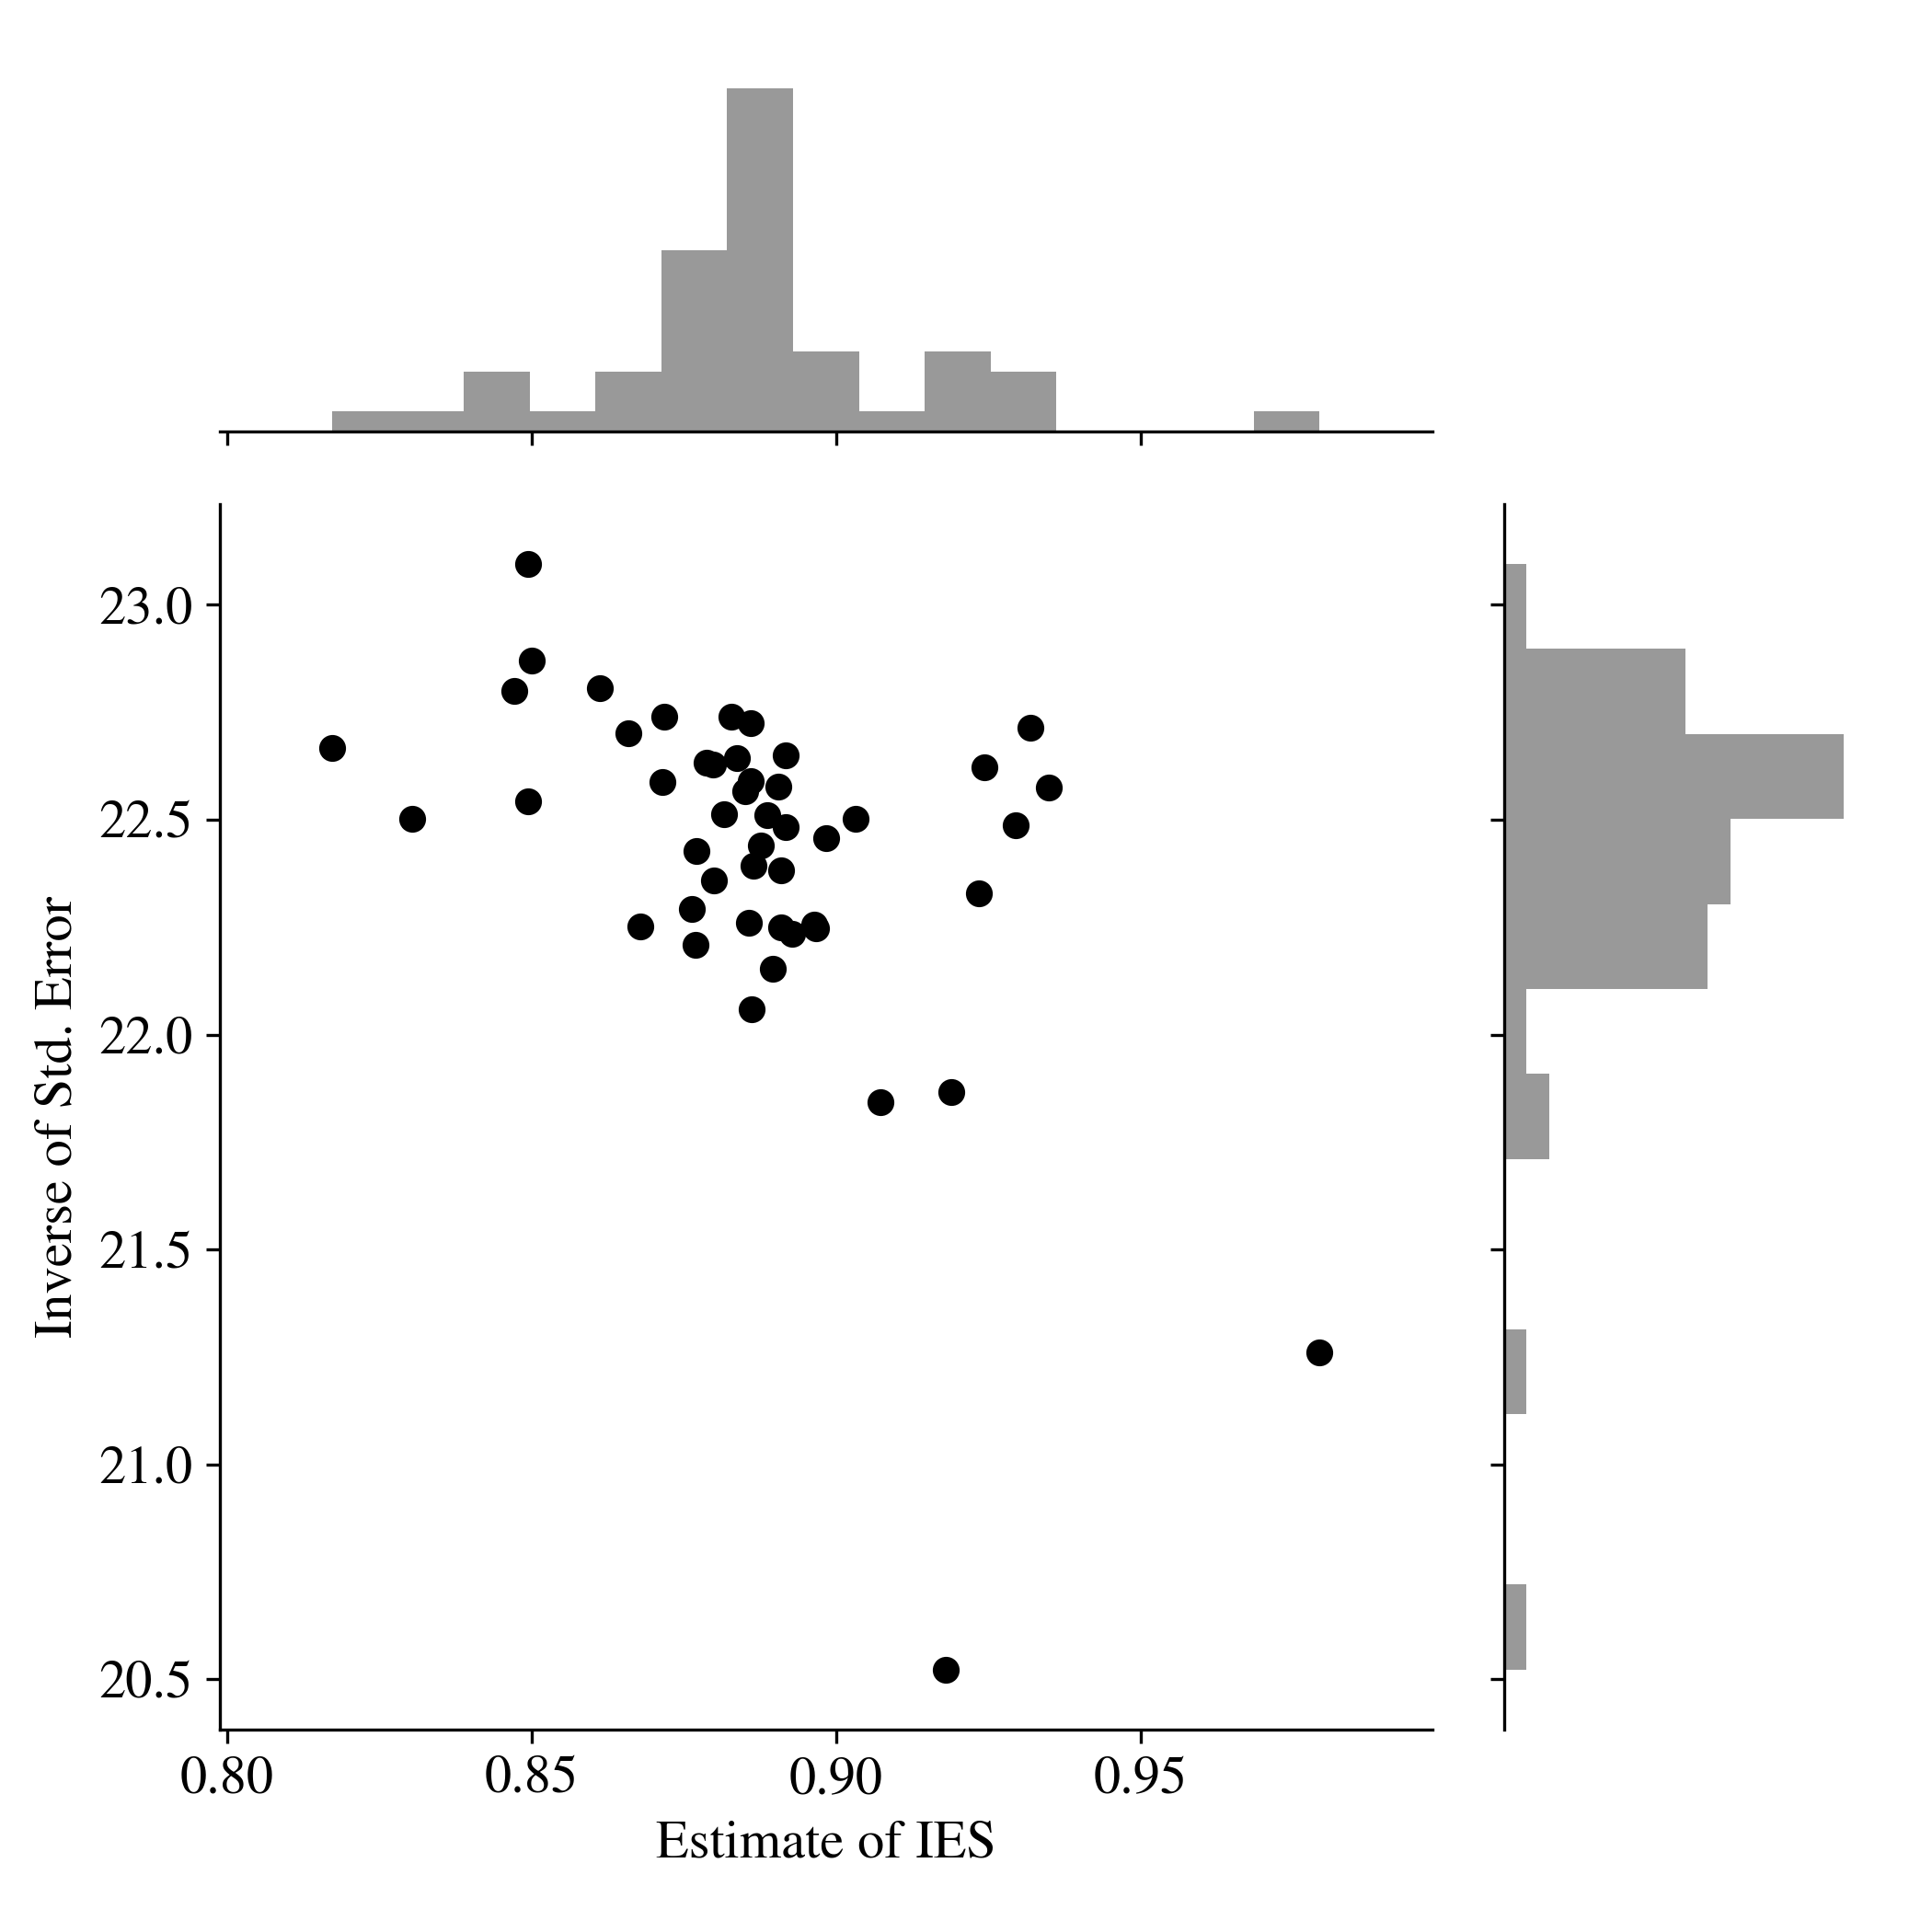
\includegraphics[width=0.75\linewidth]{../figures/regression_state_robustness_check.png} \\
			\multicolumn{1}{@{\hspace{0.2in}}p{5.9in}@{}}{ \textit{Note: } This is a joint plot of the IES  $\hat{\sigma}$ against the inverse of its estimated standard deviation from fit (3) of Table 2. Each point represents an estimate obtained from regressing on a dataset that drops out one state from the full sample. Since the sample consists of the 48 contiguous US states, this regression is a decrease in sample size of 2.08\% relative to the full dataset. On the top and right side of the graph are histograms for the two variables.}     \\  
		\end{tabular}
	\end{figure}
	\clearpage
	
	
	\begin{figure}[h!]
		\captionsetup{format=centerproper, labelformat=AppendixBFigure}
		\caption{The Elasticity of Substitution Between Two \newline  Minimally Intermittent Technologies} 
		\label{fig:eosrange}
		\footnotesize
		\vspace{-1em}
		\begin{tabular}{@{\extracolsep{0em}}c}
			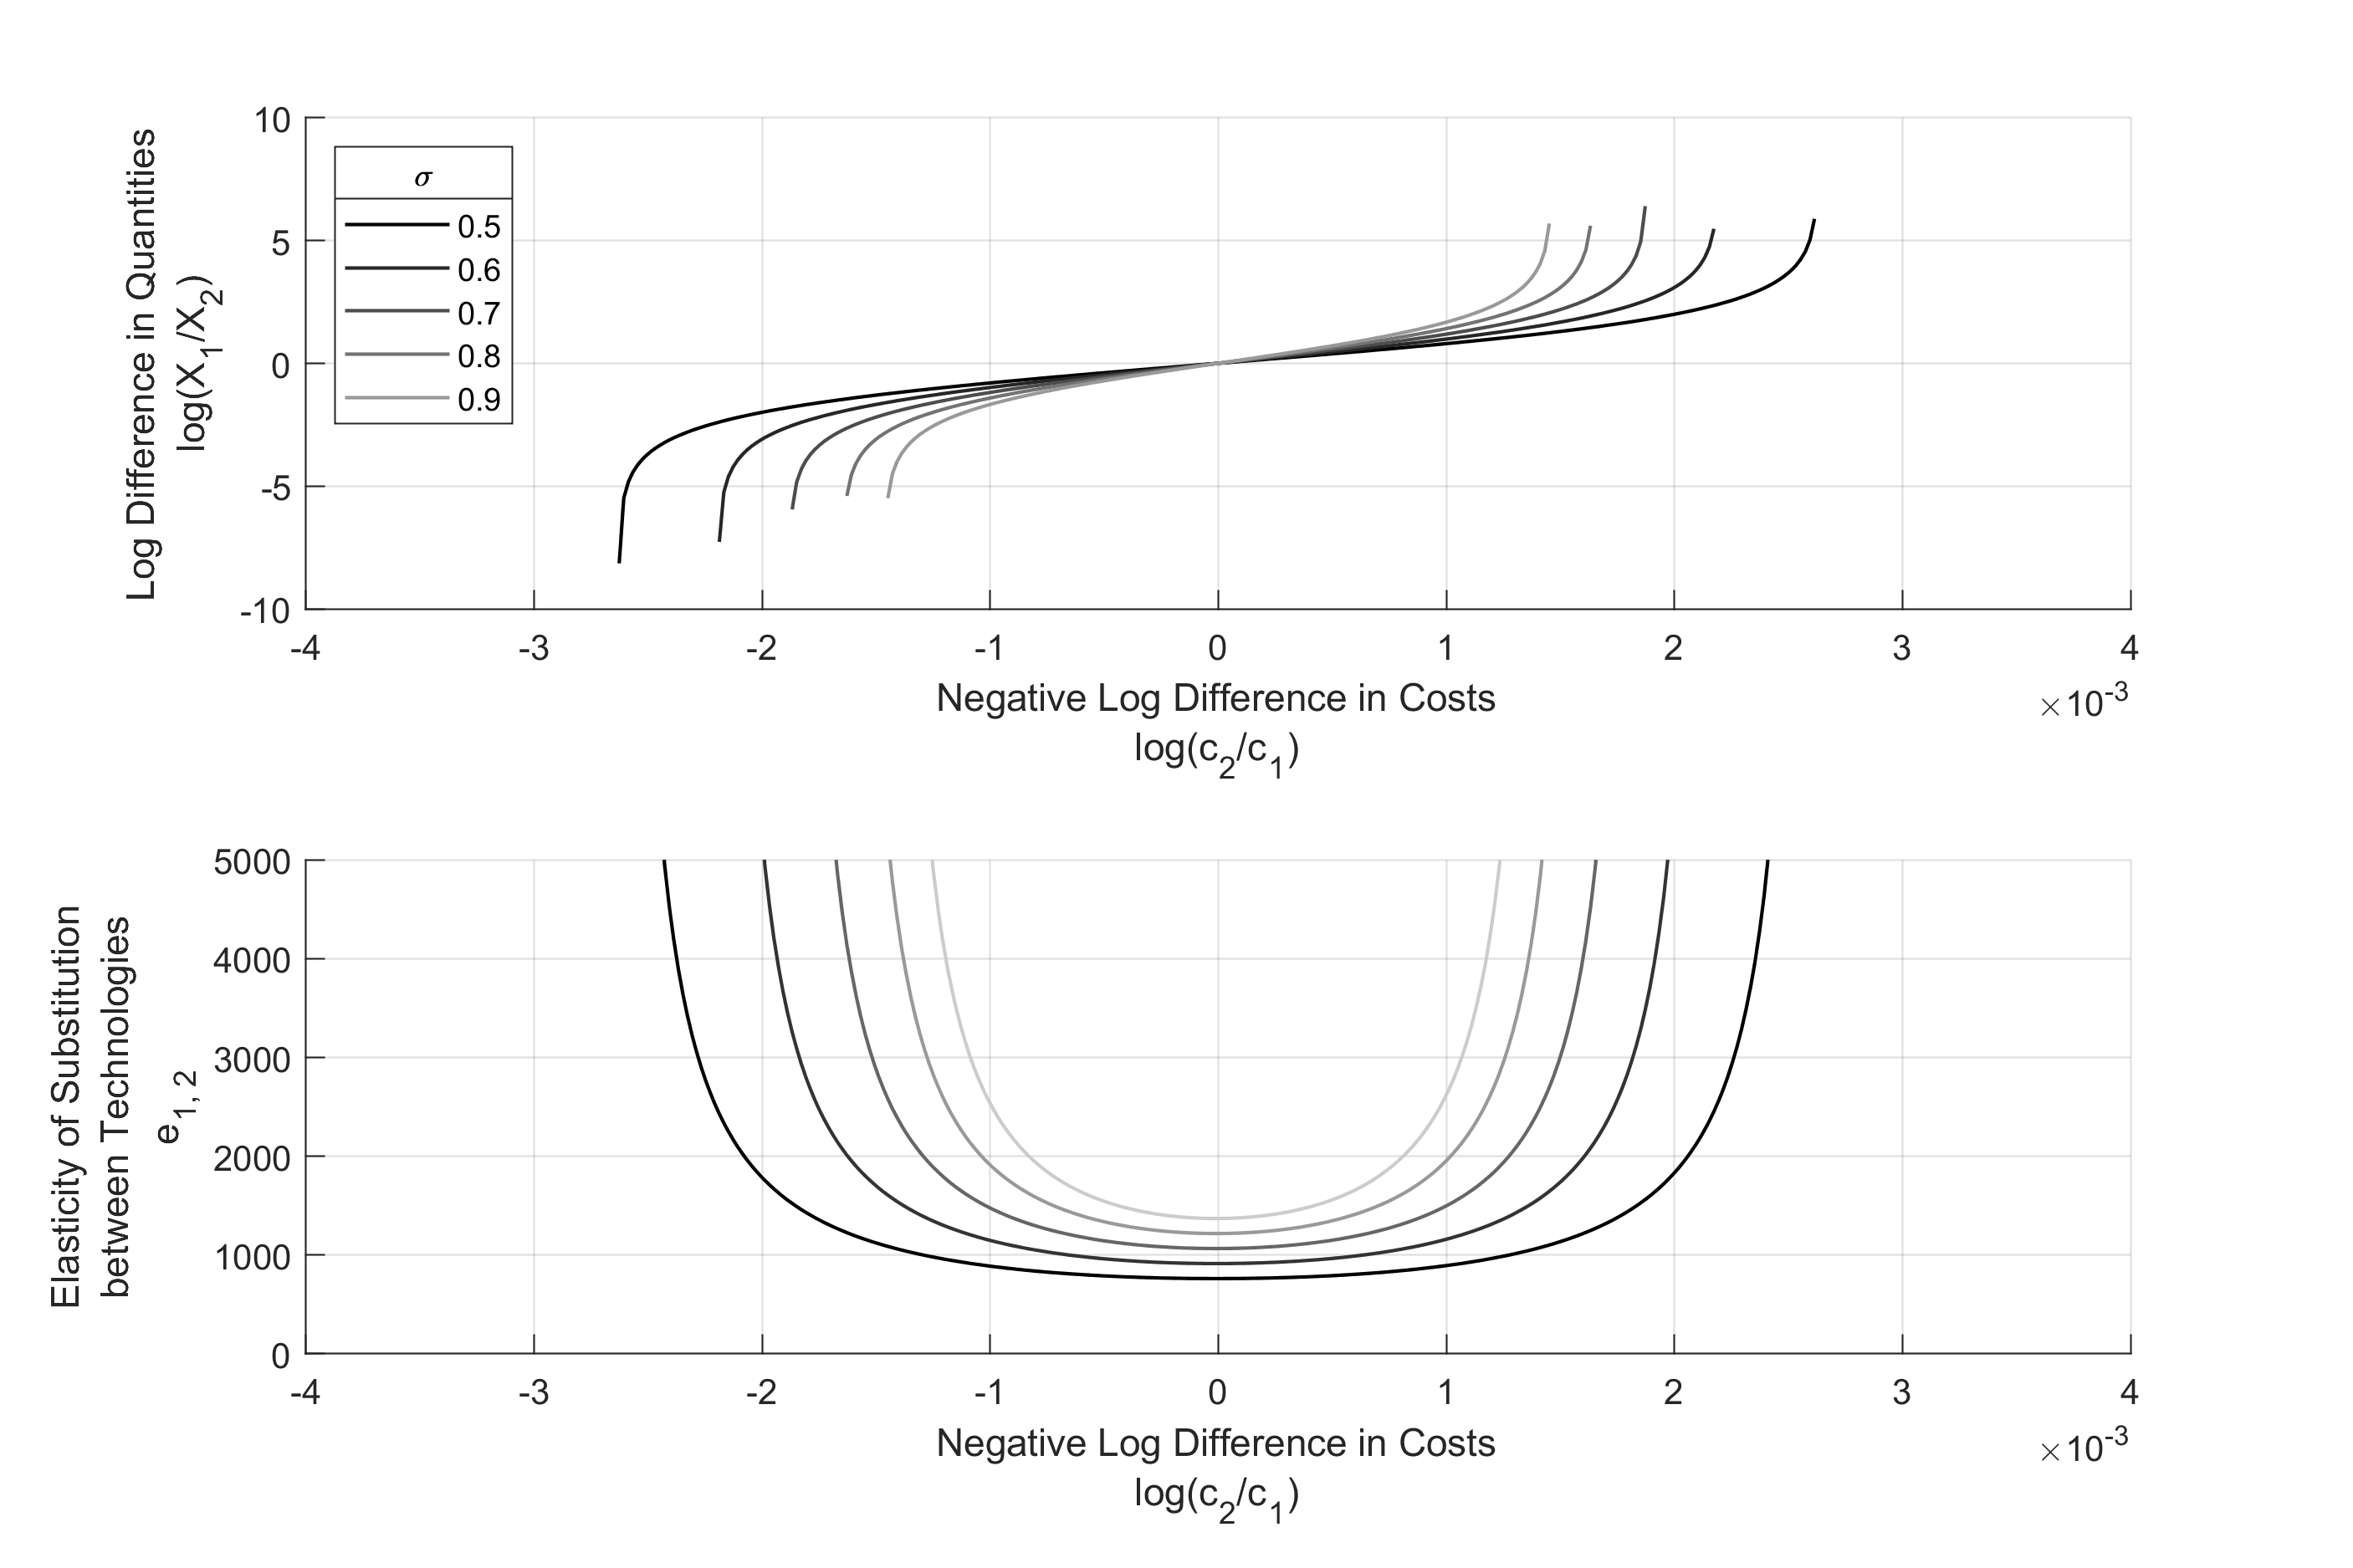
\includegraphics[width=1\linewidth]{../figures/fig_elasticity_range} \\
			\multicolumn{1}{@{\hspace{0.2in}}p{5.9in}@{}}{ \textit{Note: } The y-axis of the first plot is equivalent to $\log(X_1/X_2)$ and the x-axis of both plots is equivalent to  $\log(c_2/c_1)$. Technology 1 and 2 represent two arbitrary technologies that are practically non-intermittent. The legend in the upper subplot also applies to the lower subplot. These results were obtained using the following parameters: $\alpha_t = 0.5$, $\alpha_s = 0.5$, $\xi_1 = (0.95, \, 1)$, $\xi_2 = (1, \, 0.95)$, $c_1 = 100$, $c_2 = 100$. In order to generate these numerical results, we first found the optimal quantities of $\mathbf{X}$ over a range of prices $c_1^* \in (0.5\, c_1, 1.5 \,c_1)$. Then, we obtained estimates of the elasticity of substitution by numerically differentiating $\ln(X_1/X_2)$ with respect to $-\ln(c_1, c_2)$. That is, the elasticity of substitution  between technology 1 and 2 is given by the slope of the upper subplot, and it is graphed in the lower subplot. Finally, we repeat this procedure for various values of $\sigma$. }     \\  
		\end{tabular}
	\end{figure}
	\clearpage
	
	
	
	\begin{figure}[h!]
		\captionsetup{format=centerproper, labelformat=AppendixBFigure}
		\caption{The Elasticity of Substitution Between Coal \newline  and a Hypothetical Renewable Technology} 
		\label{fig:eosalt}
		\footnotesize
		\vspace{-1em}
		\begin{tabular}{@{\extracolsep{0em}}c}
			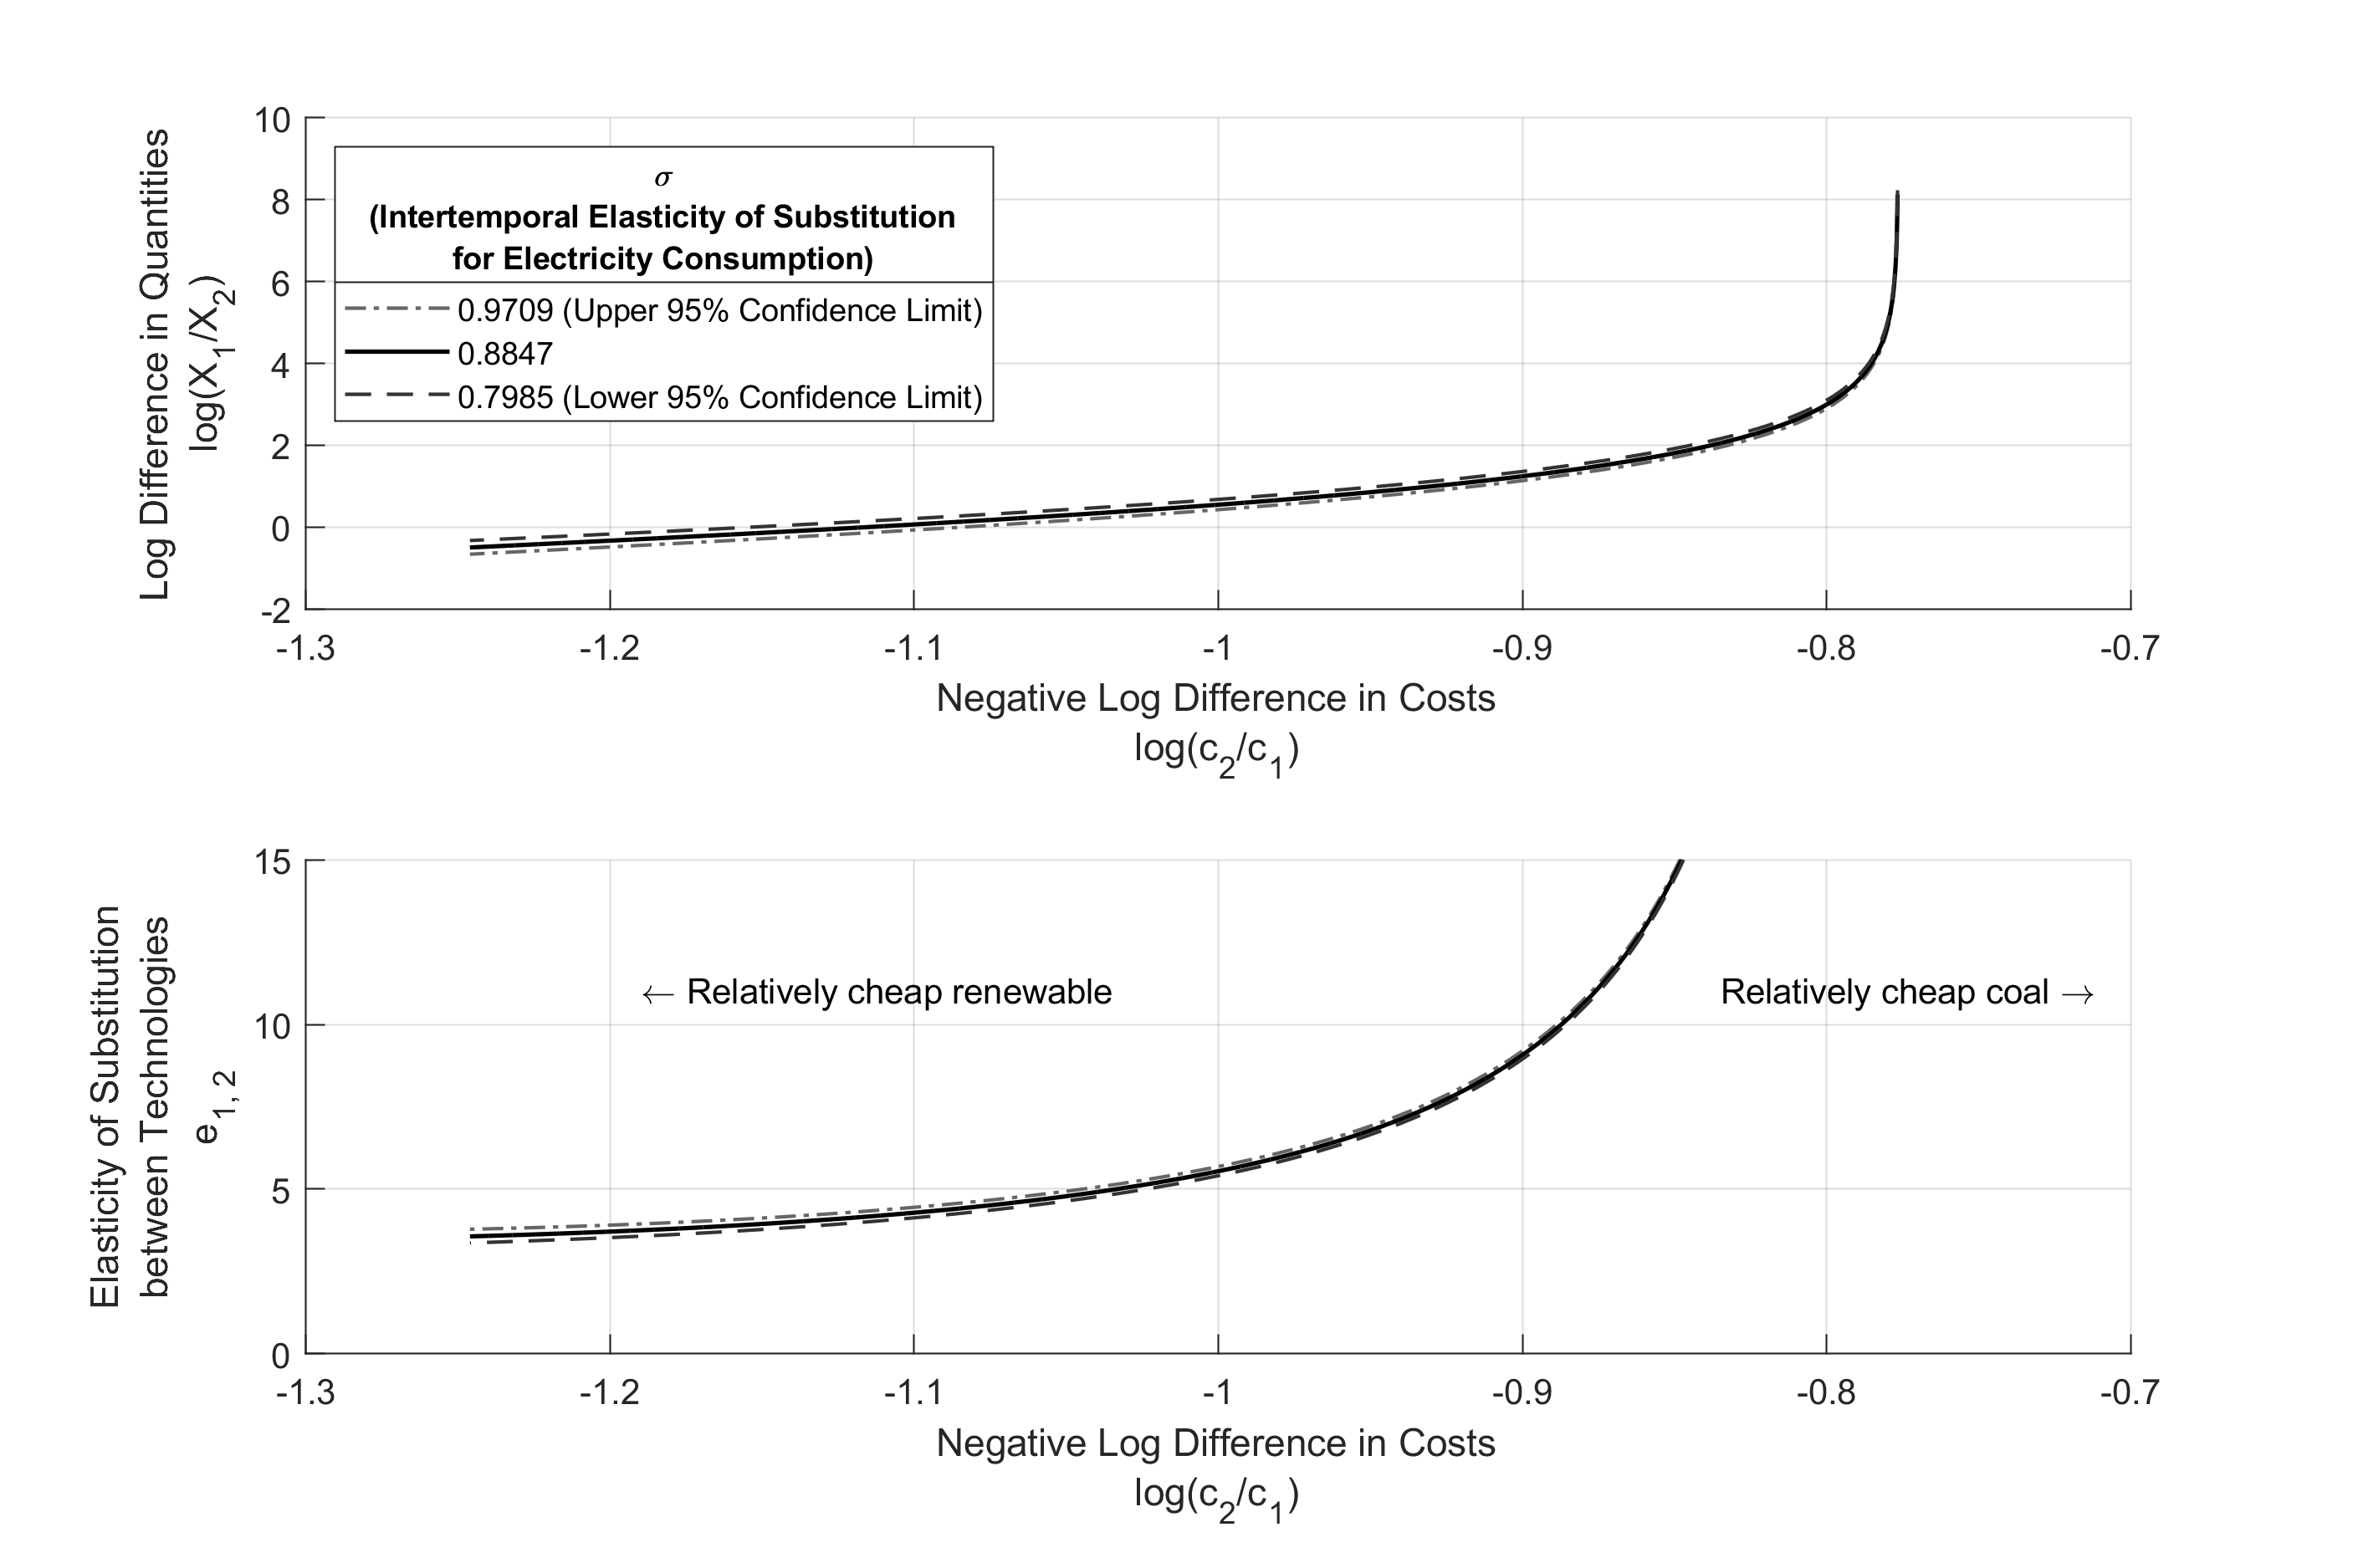
\includegraphics[width=1\linewidth]{../figures/fig_elasticity_alt} \\
			\multicolumn{1}{@{\hspace{0.2in}}p{5.9in}@{}}{\textit{Note: } Technology 1 is coal and technology 2 is a hypothetical renewable technology. This hypothetical technology has $\xi_2 = (0.1, \, 1)$ but is otherwise equivalent to solar. The legend in the upper subplot also applies to the lower subplot. These results were obtained using the following parameters: $\alpha_t = 0.6$, $\alpha_s = 0.4$, $\xi_1 = (1, \, 1)$, $\xi_2 = (0.1, \, 1)$, $c_1 = 104.3$, $c_2 = 60$. Furthermore, we set the parameter for the intertemporal elasticity of substitution for electricity consumption equal to our estimate $\hat{\sigma} = 0.8847$. In order to generate these numerical results, we first found the optimal quantities of $\mathbf{X}$ over a range of prices $c_1^* \in (0.5\, c_1, 2 \,c_1)$. Then, we obtained estimates of the elasticity of substitution by numerically differentiating $\ln(X_1/X_2)$ with respect to $-\ln(c_1/ c_2)$. That is, the elasticity of substitution  between technology 1 and 2 is given by the slope of the upper subplot, and it is graphed in the lower subplot. Finally, we repeat this procedure with $\sigma$ equal to two standard deviations above and below its estimated value $\hat{\sigma}$; that is, the dashed lines represent  $\sigma = 0.8847 \pm (1.96)(0.044)$. }     \\  
		\end{tabular}
	\end{figure}
	\clearpage
	
	\begin{figure}[h!]
		\captionsetup{format=centerproper, labelformat=AppendixBFigure}
		\caption{The VES Approximation of the Elasticity of Substitution \\ between Highly Intermittent Solar and Coal} 
		\label{fig:ves_int}
		\footnotesize
		\vspace{-1em}
		\begin{tabular}{@{\extracolsep{0em}}c}
			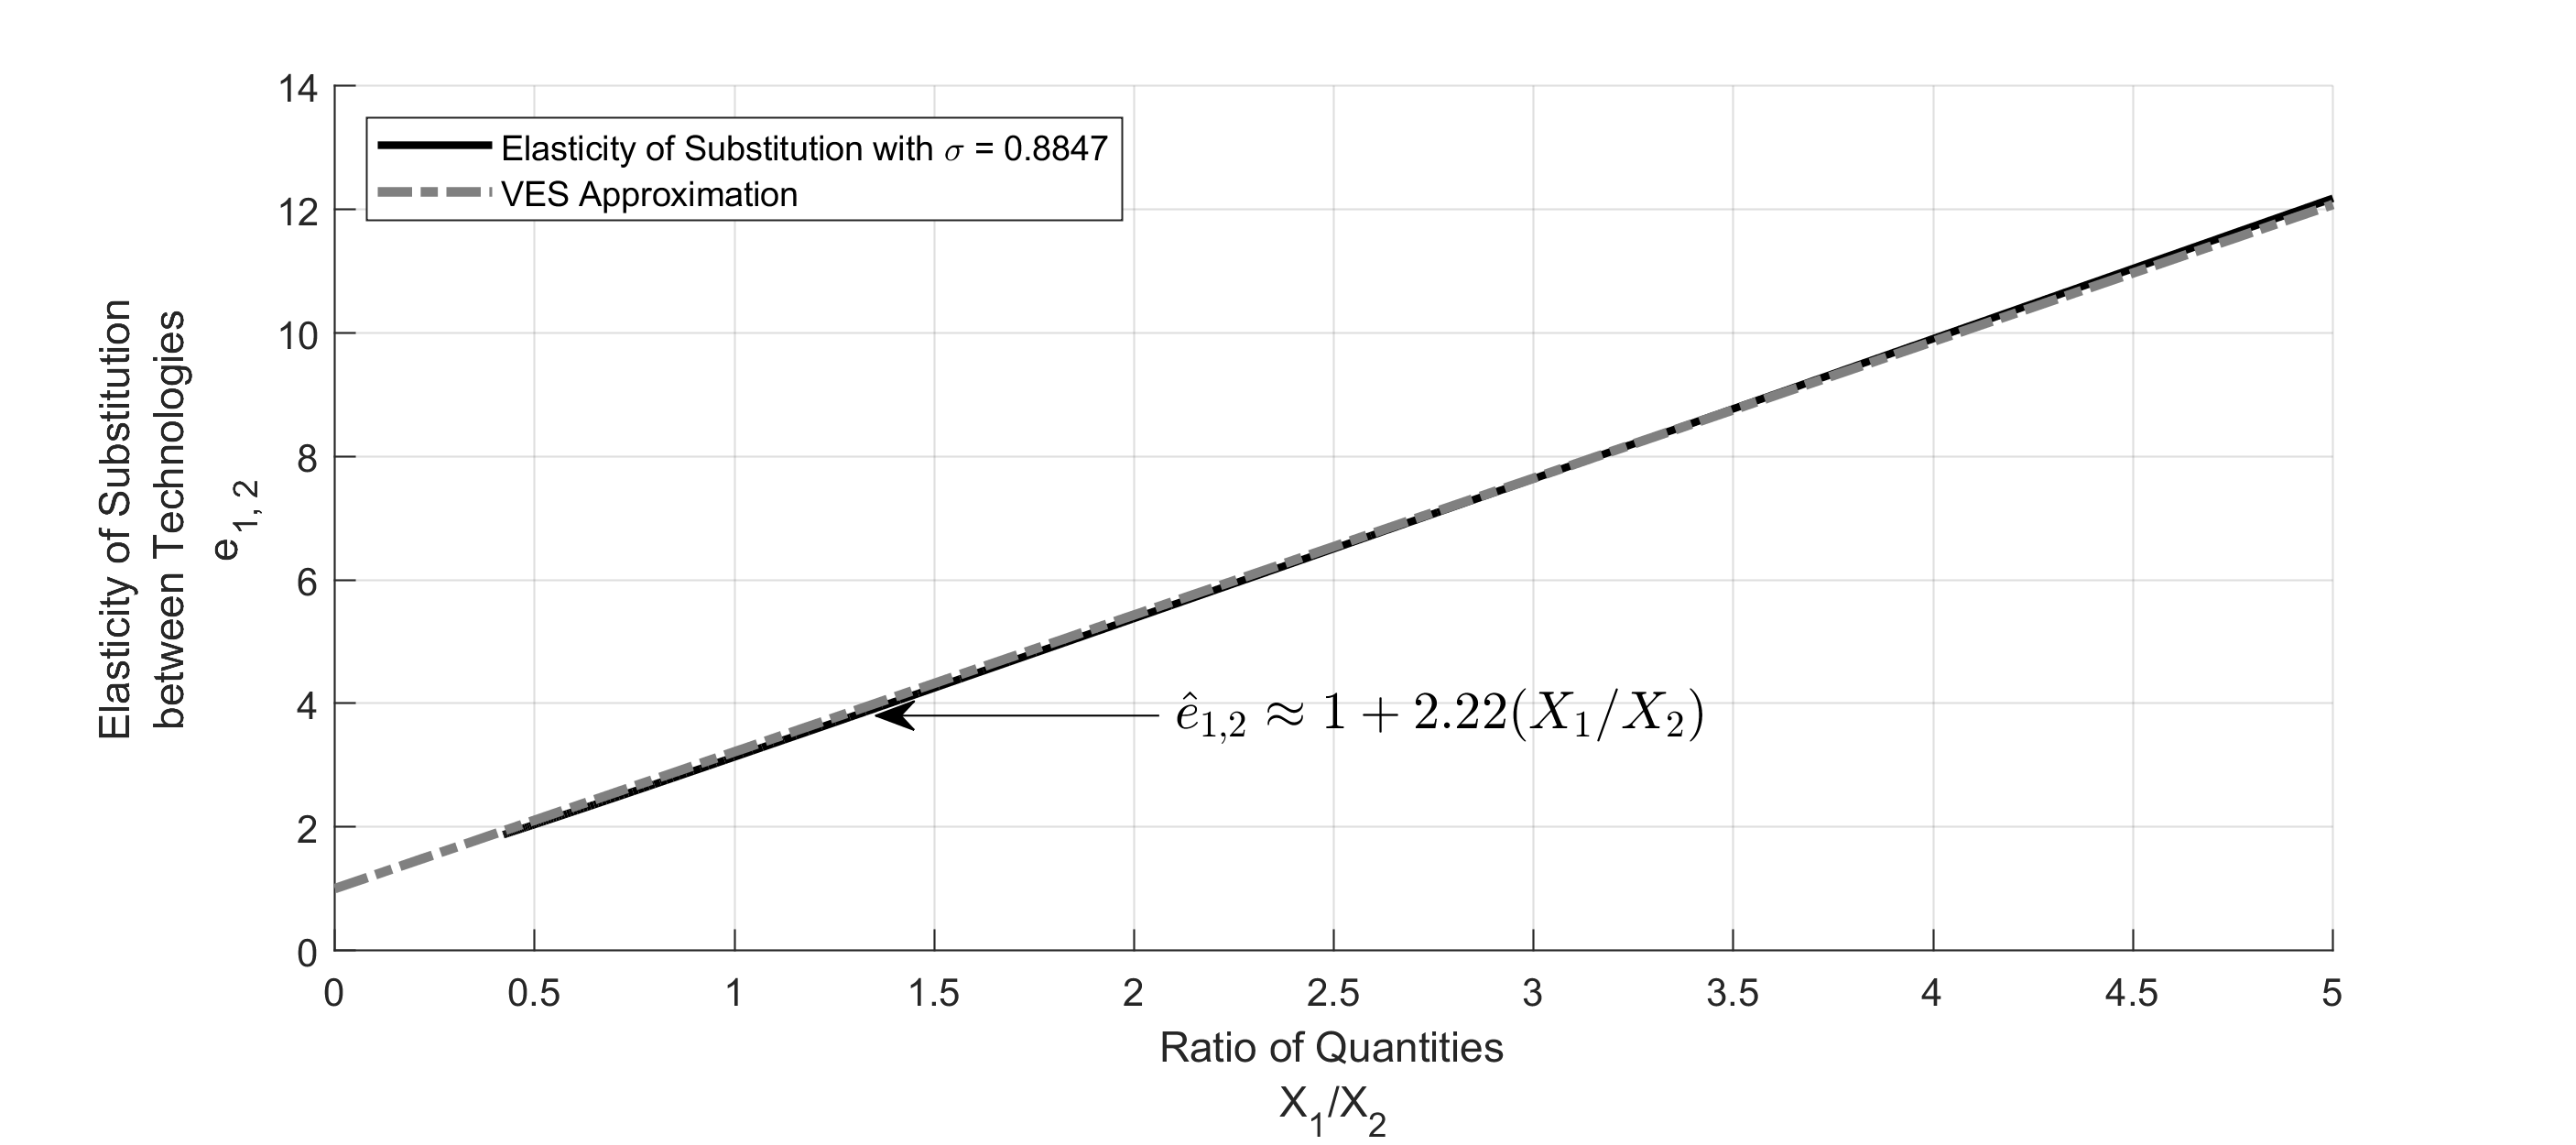
\includegraphics[width=1\linewidth]{../figures/fig_ves_approx_int} \\
			\multicolumn{1}{@{\hspace{0.2in}}p{5.9in}@{}}{ \textit{Note: } Technology 1 is coal and technology 2 is a highly intermittent version of solar. The purple, dash-dots line represents a linear approximation of $e_{1,2}$ for $\sigma = 0.8847$ with a fixed intercept of 1. These results were obtained using the following parameters: $\alpha_t = 0.6$, $\alpha_s = 0.4$, $\xi_1 = (1, \, 1)$, $\xi_2 = (1, \, 0.01)$, $c_1 = 104.3$, $c_2 = 60$. Furthermore, we set the parameter for the intertemporal elasticity of substitution for electricity consumption equal to our estimate $\hat{\sigma} = 0.8847$. In order to generate these numerical results, we first found the optimal quantities of $\mathbf{X}$ over a range of prices $c_1^* \in (c_1, 2 \,c_1)$. Then, we obtained estimates of the elasticity of substitution by numerically differentiating $\ln(X_1/X_2)$ with respect to $-\ln(c_1, c_2)$.  }     \\  
		\end{tabular}
	\end{figure}
	\clearpage
	

	
\end{document}





